\documentclass{legrand}
\usepackage{thesis_98_packages}

%-------------------------------------------------------------------------------
%	SETTING UP SOME VARIABLES :D
%-------------------------------------------------------------------------------
\def\mytitle{Analysis and implementation of an algorithm to validate Knowledge Graphs using Big data techniques} % Title of the project
\def\subtitle{From a Rustacean's perspective} % Subtitle of the project
\def\centre{Escuela de Ingeniería Informática} % The name of the center you're sitting at
\def\reviewer{Jose Emilio Labra Gayo} % reviewer of the project
\def\author{Ángel Iglesias Préstamo} % Your name.. 
\def\date{\today} % Today's date 
%-------------------------------------------------------------------------------
%-------------------------------------------------------------------------------

\begin{document}

\hypersetup{
    pdftitle={\mytitle},
    pdfauthor={\author}
}

\pagenumbering{roman}

% custom commands for use in the paper
% creating some commands for reuse later on :D
\newcommand{\myfont}[1]{\ensuremath{\mathcal{#1}}}

\newcommand{\VertSet}{\myfont{V}}
\newcommand{\NodeSet}{\myfont{N}}
\newcommand{\EdgeSet}{\myfont{E}}
\newcommand{\LabelSet}{\myfont{L}}
\newcommand{\PLabelSet}{\myfont{T}}
\newcommand{\MsgSet}{\myfont{M}}
\newcommand{\None}{\myfont{None}}

\newcommand{\triple}[3]{\ensuremath{\langle #1,#2,#3 \rangle}}
\newcommand{\quadruple}[4]{\ensuremath{\langle #1,#2,#3,#4\rangle}}
\newcommand{\ItemSet}{\myfont{Q}}
\newcommand{\PropSet}{\myfont{P}}
\newcommand{\EntitySet}{\myfont{E}}
\newcommand{\ValueSet}{\myfont{V}}
\newcommand{\DataValueSet}{\myfont{D}}
\newcommand{\StmtSet}{\rho}
\newcommand{\FinSet}[1]{\ensuremath{FinSet(#1)}}
\newcommand{\Graph}{\myfont{G}}

\newcommand{\hrefc}[3][blue]{\href{#2}{\color{#1}{#3}}}%
\newcommand{\elemento}[2]{\ensuremath{\hrefc[violet]{http://www.wikidata.org/entity/#2}{#1}}}
\newcommand{\propiedad}[2]{\ensuremath{\hrefc[blue]{http://www.wikidata.org/entity/#2}{#1}}}
\newcommand{\alanTuring}{\elemento{alanTuring}{Q7251}}
\newcommand{\wilmslow}{\elemento{wilmslow}{Q2011497}}
\newcommand{\town}{\elemento{town}{Q3957}}
\newcommand{\government}{\elemento{government}{Q220798}}
\newcommand{\warringtonLodge}{\elemento{warringtonLodge}{Q20895942}}
\newcommand{\bombe}{\elemento{bombe}{Q480476}}
\newcommand{\unitedKingdom}{\elemento{unitedKingdom}{Q145}}
\newcommand{\computer}{\elemento{computer}{Q11742076}}
\newcommand{\dateOfBirth}{\propiedad{dateOfBirth}{P569}}
\newcommand{\placeOfBirth}{\propiedad{placeOfBirth}{P19}}
\newcommand{\country}{\propiedad{country}{P27}}
\newcommand{\employer}{\propiedad{employer}{P108}}
\newcommand{\discoverer}{\propiedad{discoverer}{P61}}
\newcommand{\dateOfDeath}{\propiedad{dateOfDeath}{P570}}
\newcommand{\placeOfDeath}{\propiedad{placeOfDeath}{P20}}
\newcommand{\timeStart}{\propiedad{timeStart}{P580}}
\newcommand{\timeEnd}{\propiedad{timeEnd}{P582}}
\newcommand{\manufacturer}{\propiedad{manufacturer}{P176}}
\newcommand{\Human}{\elemento{Human}{Q5}}
\newcommand{\instanceOf}{\propiedad{instanceOf}{P31}}

\newcommand{\fb}[1]{\dofb#1}
\newcommand{\dofb}[1]{\textbf{#1}\nobreak\hspace{0pt}}

\newcommand{\mi}[1]{\ensuremath{\mathit{#1}}}

\newcommand{\emptyGraph}{\ensuremath{\emptyset}}
\newcommand{\EmptyGraph}{\ensuremath{\emptyset}}
\newcommand{\addTriple}{\ensuremath{\rtimes}}
\newcommand{\unionGraphs}{\ensuremath{\cup}}
\newcommand\neighs[2]{\ensuremath{neighs(#1,#2)}}
\newcommand\nodes[1]{\ensuremath{nodes(#1)}}
\newcommand{\node}{\mi{n}}
\newcommand{\lbl}{\mi{l}}
\newcommand{\g}{\mi{g}}
\newcommand{\vertex}{\mi{v}}
\newcommand{\msg}{\mi{msg}}
\newcommand{\msgs}{\mi{msgs}}
\newcommand{\WShape}{\mi{WShape}}
\newcommand{\WShapeRef}{\mi{WShapeRef}}
\newcommand{\WShapeComposite}{\mi{WShapeComposite}}
\newcommand{\WShapeLiteral}{\mi{WShapeLiteral}}

% Algorithmic definitions
\SetKwProg{Def}{def}{$\,$:}{}
\SetKwProg{Defn}{def}{~$=$}{}
\SetKw{defn}{def}
\newcommand{\DefInline}[2]{\defn #1 = #2}
\SetKwProg{DefnCustom}{\defn}{}{}
\SetKw{Let}{let}
\SetKwInput{KwIn}{Input}
\SetKwFor{ForEach}{foreach}{}{}
\SetKw{Or}{or}
\SetKw{And}{and}
\SetKwIF{If}{ElseIf}{Else}{if}{then}{else if}{else}{endif}
\SetKw{Match}{match}
\SetKw{MyIf}{if}
\SetKw{MyThen}{then}
\SetKw{MyElse}{else}
\SetKw{Case}{case}
\SetKwBlock{Let}{let}{in}
\SetKw{In}{in}
\SetKw{MapTo}{\ensuremath{\;\;\Rightarrow\;\;}}
\SetKwBlock{Block}{}{}
\newcommand{\assign}{\ensuremath{~\mathtt{:=}~}}
\newcommand{\algocomment}[1]{\text{//$\,$#1}}

\newcommand{\blockskip}{\smallskip}
\newcommand{\done}{\ensuremath{\mathit{done}}}

% [algorithm spacing:]
\def\algorithmsize{small}
\def\algorithmheadersize{\algorithmsize}
\renewcommand\AlCapFnt{\normalfont\bfseries\small}
\setlength{\textfloatsep}{1.0ex}
\setlength{\floatsep}{1.0ex}

% Statuses
\newcommand{\Ok}{\ensuremath{Ok}}
\newcommand{\Failed}{\ensuremath{Failed}}
\newcommand{\WaitingFor}[3]{\ensuremath{WaitingFor}(#1,#2,#3)}
\newcommand{\Pending}{\ensuremath{Pending}}
\newcommand{\PendingLs}{\ensuremath{Pending}(ls)}
\newcommand{\Undefined}{\ensuremath{Undefined}}

\newcommand{\Validate}{\ensuremath{Validate}}
\newcommand{\Checked}[2]{\ensuremath{Checked(#1,#2)}}
\newcommand{\WaitFor}[1]{\ensuremath{WaitFor(#1)}}
\newcommand{\status}[2]{\ensuremath{#1(#2)}}
\newcommand{\msgSent}[3]{\ensuremath{#1,#2\rightsquigarrow{}#3}}
\newcommand{\checkLocal}[2]{\ensuremath{checkLocal(#1,#2)}}
\newcommand{\checkLocalOpen}[2]{\ensuremath{checkLocalOpen(#1,#2)}}

\newcommand{\checkNeighs}[3]{\ensuremath{checkNeighs}(#1,#2,#3)}
\newcommand{\fracEmpty}[2]{\genfrac{}{}{0pt}{0}{#1}{#2}}
\newcommand{\vProg}{vProg}
\newcommand{\tripleConstraints}[1]{tripleConstraints(#1)}
\newcommand{\rbe}[1]{\ensuremath{rbe(#1)}}
\newcommand{\combine}[2]{\ensuremath{combine(#1,#2)}}

\chapterimage{img/misc/heading_main.pdf} % Chapter heading image
\begin{titlepage}
    %
    %
    \begin{figure*}[ht]
        \includegraphics[width=0.5\textwidth]{img/logo_header.png}
    \end{figure*}

    \vspace{10mm}
    \hbox{ % Horizontal box
    \hspace*{0.08\textwidth} % Whitespace to the left of the title page
    \rule{1.5pt}{0.80\textheight} % Vertical line
    \hspace*{0.02\textwidth} % Whitespace between the vertical line and title page text
    \parbox[b]{0.90\textwidth}{ % Paragraph box which restricts text to less than the width of the page


    {\large \textsc{Final Degree Project}}\\[\baselineskip] % Tagline or further description
    \begin{flushleft}
        {\Large\bfseries Analysis and implementation of an algorithm to validate Knowledge Graphs using Big data techniques}\\[2\baselineskip] % Title
    \end{flushleft}

    {\Large Ángel Iglesias Préstamo}\\ % Author name
    {\large \it Supervised by Jose Emilio Labra Gayo}\\[3\baselineskip] % Supervisor name

    \vspace{0.15\textheight} % Whitespace between the title block and the publisher
    {\noindent University of Oviedo 2022-23}\\[\baselineskip] % Publisher and logo
    }}
    %
    %
\end{titlepage}

% include the abstract, written in a separate file called thesis_02_abstract.tex
\setcounter{page}{0}
\newenvironment{abstract}%
{\cleardoublepage\null\vfill\section*{\abstractname}}%
{\vfill\null}
\begin{abstract}
    The necessity of processing large amounts of data is getting increased with the time. Not only we need to process high volumes of sequential information, but more complex structures such as graphs. One of the sources we can retrieve data from is Wikidata, the central storage for the structured data of the Wikimedia projects: including Wikipedia. The shape of the documents to be processed from Wikidata tends to be heterogeneous: the structure of a human node may vary from the one of a mountain. More in more, it could be handful to generate subsets out of a dump in order us to work with concrete nodes.
\end{abstract}

\noindent \textbf{Keywords} --- \textit{Knowledge Graphs, RDF, Linked Data, RDF Validation, Shape Expressions, Subsets, MapReduce, Pregel, Algorithms, Wikibase, Apache Spark, Scala, Rust, DuckDB.}
% print no page number
\thispagestyle{empty}
\phantom{~}
\vspace{40mm}
\begin{flushright}
    {\em
        Data is a precious thing\\[0.25\baselineskip]
        and will last longer than the systems themselves\\[1.5\baselineskip]
        --Tim Berners-Lee
    }
\end{flushright}

\vfill

% Create a table of contents - not mandatory
\pdfbookmark{\contentsname}{toc}
\tableofcontents

% Create a list of figures
\listoffigures

% Create a list of tables
\listoftables


\chapter{Introduction}
% and we establish the numeration back to the normal one 
\setcounter{page}{0} % reset numbering to 1, 2, 3...
\pagenumbering{arabic}
\label{chapter:intro}
\epigraph{\textit{We cannot solve problems with the kind of thinking we employed when we came up with them.}}{-- \textup{Albert Einstein}}

During the following paragraphs I am covering the motivation, contributions and structure of this document. This means, after reading it, you are building the big picture; a general idea of the motivations to develop this project, the results we are looking for and the shape of it.

\section{Motivation}

These days, a growing number of devices are interconnected. As a result, a ton of data is being automatically stored. This way, processing that data becomes both a more challenging procedure and a more important task. Simply stated, the amount of data outruns our capacity to consume it. Big data, a new area of software development where we quickly handle large volumes of heterogeneous information, offers a remedy for this.

Interoperability is a crucial subject we must deal with in big data applications since they not only need to scan huge volumes of inputs as quickly as possible but also because information comes from a range of sources.

Knowledge graphs~\cite{https://doi.org/10.48550/arxiv.2110.11709} were popularized back in 2012 by Google~\cite{web:knowledge_graphs:google} as a tool to represent real world data reflecting relationships between entities in order to understand those links better. After Google's introduction, others embraced this approach: ranging from proprietary to open databases. Being the content of the latter publicly available. Prominent companies -- including \textit{web search} (e.g., Bing~\cite{knowledge:graphs:usage:bing} and Google~\cite{web:knowledge_graphs:google}), \textit{commerce} (e.g., Airbnb~\cite{knowledge:graphs:usage:airbnb} and Amazon~\cite{knowledge:graphs:usage:amazon}), \textit{social networks} (e.g., Facebook~\cite{knowledge:graphs:usage:facebook} and LinkedIn~\cite{knowledge:graphs:usage:linkedin}) or \textit{finances} (e.g., Accenture~\cite{knowledge:graphs:usage:accenture} and Banca d'Italia~\cite{https://doi.org/10.48550/arxiv.2010.05172}) -- are using knowledge graphs in order to have a better understanding of their customers. Even though there exist several models associated with this technology, we are focusing on Wikibase graphs.

Summing up, this project focuses on the analysis and implementation of a system to validate Wikibase graphs -- a specific flavor of the so-called knowledge graphs -- using big data techniques. To put that into perspective, as of October 1, 2022, a compressed \gls{dump} of Wikidata's database has a size of 109.04Gb~\cite{wikidata:dumps}. Not only that, but the size of these dumps has exponentially increased with each and every release of a new one (see Figure \ref{fig:dumps}).

These enormous sizes have the effect of making it difficult for users to easily examine and process the content, and they also raise the possibility that these technologies will become victims of their own success. This condition is demonstrated in Scholia, an online application that uses Wikidata to describe data about academics and their works. Additionally, the app includes appealing visualizations and comparisons that are based on requests through the Wikidata endpoint. Despite the project offering a wealth of intriguing data, timeouts caused by the massive volumes of data prevent access to the most intricate visualizations.

Creating subsets of the Knowledge Graphs for specific domains may be one solution to these problems. These subsets serve as snapshots of the data at certain points in time and be used to enhance the performance of the apps that use that data, making it easier to do research on the contents of Knowledge Graphs.

\begin{figure}[ht]
    \centering
    \includestandalone{figures/fig_01_dumps}
    \caption[Plot showing the size of compressed dumps between 2014-22]{Size of compressed Wikidata dumps between 2014-2022~\cite{https://doi.org/10.48550/arxiv.2110.11709}}
    \label{fig:dumps}
\end{figure}

\paragraph{Project's Goal 1}
\textit{Design and implementation of a system for validating huge dumps from Wikidata generating a subset out of it.} As we have stated during these introductory lines, the task of having to process enormous amounts of data is becoming increasingly relevant. The faster a system allows us to accomplish it, the better solution we will provide.

\paragraph{Project's Goal 2}
\textit{Reproduce an experiment related to the analysis of the previously described algorithm.} In order us to properly analyze the results emerging from the execution of the algorithm we have implemented, we have to create an ecosystem were we can obtain information related to memory consumption or execution time, to name a few.

\paragraph{Project's Goal 3}
\textit{Learn new technologies and Big data techniques.} This is an academic project, not only that, but one of the main objectives of researching is finding new solutions to a certain problem. This means, learning and exploring new possibilities is -- indeed -- one goal of this project.

\section{Contributions}

The main contributions of this project are:

\begin{enumerate}
    \item
\end{enumerate}

\section{Structure of the document}

The shape of this document is as follows:

\begin{itemize}
    \item \textbf{Chapter ~\ref{chapter:description}.} General description of the existing technologies related to knowledge graph validation. As well as the advantages and disadvantages of choosing some tools over others for implementing this project.
    \item \textbf{Chapter ~\ref{chapter:theory}.} Provides a theoretical background needed for better understanding the concepts explained in the following chapters.
    \item \textbf{Chapter ~\ref{chapter:experiment}.} Explanation of the process followed to analyze the concrete implementation of the algorithm that we used to validate the knowledge graphs.
    \item \textbf{Chapter ~\ref{chapter:results}.} Analysis of the results obtained from the previously described experiment.
    \item \textbf{Chapter ~\ref{chapter:conclusions}.} Summary of the general conclusions and future work.
\end{itemize}

\chapter{State of the art}
\label{chapter:related}
\epigraph{\textit{If I have seen further, it is by standing on the shoulders of giants.}}{-- \textup{Isaac Newton}}

Some work has already been done in the field of Knowledge graph validation. In this section we are exploring what other projects have achieved and their limitations.

\section{Bid data processing and graphs}

Having to process enormous graphs made Google propose Pregel~\cite{10.1145/1807167.1807184} a model for large-scale graph computing, back in 2010. Following the idea of \textit{think like a vertex}, other systems were introduced: GraphLab~\cite{10.14778/2212351.2212354}, PowerGraph~\cite{180251} or GraphX~\cite{186216}. Being the latter a framework that enables the implementation of parallel computing algorithms.

\section{Knowledge graphs}

This article is closely related to Labra's paper~\cite{https://doi.org/10.48550/arxiv.2110.11709} on utilizing Shape Expressions to generate knowledge graph subsets, where he described the approach used in this document as one of the potential implementations. MARS (Multi-Attributed Relational Structures)~\cite{ijcai2017p165}, which are a generalized concept of property graphs, are the source of inspiration for our description of Wikibase graphs. They also define MAPL (Multi-Attributed Predicate Logic) as a formalism of logic that may be applied to ontological reasoning in that work.

\section{Knowledge graph descriptions}

\section{Knowledge graph subsets}

\chapter{Theoretical Background}
\label{chapter:theory}
\epigraph{\textit{It doesn't matter how beautiful your theory is, it doesn't matter how smart you are. If it doesn't agree with experiment, it's wrong.}}{-- \textup{Richard P. Feynman }}

\section{Knowledge graph}

A knowledge graph uses a graph-structured data model to represent knowledge of some real-world domain. Where each node represents an entity -- a \textit{thing} from the actual world -- and the edges are the relationships between them. This type of graphs are often assembled from a wide variety of sources, and as a result, can be highly diverse in terms of structure and granularity~\cite{DBLP:journals/corr/abs-2003-02320}. To address this issue, representations of \textit{schema}, \textit{identity} and \textit{context} are needed. While the former defines the high-level structure of the graph, \textit{identity} relates nodes that conform the same real-world entity; finally, \textit{context} provides the environment for a specific knowledge to be understood. These graphs can be represented using different technologies; however, we will focus on attributed graphs.

\subsection{Wikibase graphs}

Wikidata started back in 2012 as a support to Wikipedia. Rapidly becoming one of the biggest human knowledge bases, with remarkable organizations donating their data to it; as an example, Google migrated \textit{Freebase} -- its previous knowledge graph -- to Wikipedia in 2014~\cite{10.1145/2872427.2874809}. As of October 9 2022, Wikidata currently contains roughly 100 million items\footnote{\url{https://www.wikidata.org/wiki/Wikidata:Statistics}}. Internally, Wikidata's content is stored in a SQL database (MariaDB); however, this system is not ideal for querying or data analysis. With that in mind, and pursuing the integration of Wikibase within the semantic web ecosystem, the Wikimedia Foundation adopted BlazeGraph: an open-source triple store and graph database\footnote{\url{https://en.wikipedia.org/wiki/Blazegraph}}. This way, two data models coexist in Wikibase: a document-centric model based on MediaWiki and an RDF-based one that can be used to perform SPARQL queries through the Query Service~\cite{https://doi.org/10.48550/arxiv.2110.11709}.

\begin{figure}[h]
    \centering
    \includestandalone{figures/architecture_wikibase}
    \caption[Simplified architecture of Wikibase]{Simplified architecture of Wikibase~\cite{https://doi.org/10.48550/arxiv.2110.11709}}
    \label{fig:architecture:wikibase}
\end{figure}

Informally speaking, the Wikibase data model is composed by \textit{entities} and \textit{statements} (about those entities). This way, an entity can be either an \textit{item} or a \textit{property}. Items are used to represent all the \textit{things} from the human knowledge. Usually denoted by a \texttt{Q} followed by an identifier; for example, \href{https://www.wikidata.org/wiki/Q7251}{Q7251} represents Alan Turing in Wikidata. On the other hand, properties model a relationship between an item and a value, and are represented by a \texttt{P} followed by its identifier; as an example, \href{https://www.wikidata.org/wiki/Property:P31}{P31} is the property \textit{instance of} in Wikidata.

For values to be associated to properties, they must belong to some specific data types\footnote{\url{https://www.wikidata.org/wiki/Help:Data_type}}. Supported data types include: URLs, time, quantities, mathematical expressions; to name a few.

Lastly, an statement is a piece of data about an item\footnote{\url{https://www.wikidata.org/wiki/Help:Statements}} that is recorded in the page of the item itself. Putting it all together, the way Wikibase manages information is as follows: through an statement, we add information to a certain item using some property and its value. An example to that is:

\begin{table}[ht]
    \centering
    \begin{tabular}{|c|l|l|l|}
        \hline
        \rowcolor[HTML]{EFEFEF}
        \textbf{Language}     & \multicolumn{1}{c|}{\cellcolor[HTML]{EFEFEF}\textbf{Item}}                              & \multicolumn{1}{c|}{\cellcolor[HTML]{EFEFEF}\textbf{Property}}                            & \multicolumn{1}{c|}{\cellcolor[HTML]{EFEFEF}\textbf{Value}}                             \\ \hline
        \textit{English}      & \multicolumn{1}{l|}{\href{https://www.wikidata.org/wiki/Q11678}{The Hunger Games}}      & \multicolumn{1}{l|}{\href{https://www.wikidata.org/wiki/Property:P136}{genre}}            & \multicolumn{1}{l|}{\href{https://www.wikidata.org/wiki/Q15062348}{dystopian fiction}}  \\ \hline
        \textit{Spanish}      & \multicolumn{1}{l|}{\href{https://www.wikidata.org/wiki/Q11678}{Los juegos del hambre}} & \multicolumn{1}{l|}{\href{https://www.wikidata.org/wiki/Property:P136}{género}}           & \multicolumn{1}{l|}{\href{https://www.wikidata.org/wiki/Q15062348}{ficción distópica}}  \\ \hline
        \textit{French}       & \multicolumn{1}{l|}{ \href{https://www.wikidata.org/wiki/Q11678}{Hunger Games}}         & \multicolumn{1}{l|}{\href{https://www.wikidata.org/wiki/Property:P136}{genre artistique}} & \multicolumn{1}{l|}{\href{https://www.wikidata.org/wiki/Q15062348}{fiction dystopique}} \\ \hline
        \multicolumn{1}{l|}{} & \multicolumn{1}{c|}{\href{https://www.wikidata.org/wiki/Q11678}{Q11678}}                & \multicolumn{1}{c|}{\href{https://www.wikidata.org/wiki/Property:P136}{P136}}             & \multicolumn{1}{c|}{\href{https://www.wikidata.org/wiki/Q15062348}{Q15062348} }         \\ \cline{2-4}
    \end{tabular}
    \caption[Including information about the genre of \textit{The Hunger Games}]{\label{tab:wikibase:graph}Including information about the genre of \textit{The Hunger Games}\footnote{\url{https://www.wikidata.org/wiki/Q11678}}}
\end{table}

This way, what we are achieving is a database where we link concepts in a language-agnostic approach. Notice that in the previous example there is only one \textit{statement} which relates the \textit{item} \texttt{Q11678} with the \textit{value} \texttt{Q15062348} through the \textit{property} \texttt{P136}. Instead of storing attributes that are language-dependent; following this example, The \textit{statement} $s = \{ (\href{https://www.wikidata.org/wiki/Q11678}{Q11678}, \href{https://www.wikidata.org/wiki/Property:P136}{P136}, \href{https://www.wikidata.org/wiki/Q15062348}{Q15062348}, \{\}) \}$ is equivalent to: \textit{the genre of The Hunger games is dystopian fiction}. What we are doing is linking concepts.

\begin{definition}[Wikibase graph~\cite{https://doi.org/10.48550/arxiv.2110.11709}]
    Given a mutually disjoint set of items \ItemSet{}, a set of properties \PropSet{} and a set of data values \DataValueSet{}, a \emph{Wikibase graph} is a tuple $\langle\ItemSet,\PropSet,\DataValueSet,\StmtSet\rangle$ such that $\StmtSet\subseteq\EntitySet\times\PropSet\times\ValueSet\times\FinSet{\PropSet\times\ValueSet}$ where $\EntitySet=\ItemSet\cup\PropSet$ is the set of entities which can be subjects of a statement and $\ValueSet=\EntitySet\cup\DataValueSet$ is the set of possible values of a property.
\end{definition}

For better understanding this formal definition, let me explain it step-by-step. First, let us clarify what the described symbols are: $\mathcal{Q}$ is the set containing the different entities (\textit{things}), $\mathcal{P}$ is the set with the different possible relationships in the graph, $\mathcal{D}$ is the set containing data values and $\rho$ is the set where each element represents a relation between two entities and a certain data value. Having that said, we can now see an example for further clarifications:

\begin{longtable}{ccl}
    \ItemSet      & = \{ & \alanTuring, \wilmslow, \government, \unitedKingdom, \warringtonLodge,                           \\
                  &      & \bombe, \town, \computer \hspace{1mm} \}                                                         \\
    \PropSet      & = \{ & \dateOfBirth, \placeOfBirth, \employer, \dateOfDeath, \placeOfDeath,                             \\
                  &      & \timeStart, \country, \timeEnd, \manufacturer, \instanceOf \hspace{1mm} \}                       \\
    \DataValueSet & = \{ & {\small 23 June 1912}, {\small 7 June 1954}, {\small 1938}, {\small 1945}\hspace{1mm} \}         \\
    $\StmtSet$    & = \{ & (\alanTuring, \instanceOf, \Human, \{\}),                                                        \\
                  &      & (\alanTuring, \dateOfBirth, {\small 23 June 1912}, \{\}),                                        \\
                  &      & (\alanTuring, \placeOfBirth, \warringtonLodge, \{\}),                                            \\
                  &      & (\alanTuring, \dateOfDeath, {\small 7 June 1954}, \{\}),                                         \\
                  &      & (\alanTuring, \placeOfDeath, \wilmslow, \{\}),                                                   \\
                  &      & (\alanTuring, \employer, \government, \{ \timeStart: {\small 1938}, \timeEnd: {\small 1945} \}), \\
                  &      & (\bombe, \discoverer, \alanTuring, \{\}),                                                        \\
                  &      & (\bombe, \manufacturer, \government, \{\}),                                                      \\
                  &      & (\bombe, \instanceOf, \computer, \{\}),                                                          \\
                  &      & (\bombe, \country, \unitedKingdom, \{\})                                                         \\
                  &      & (\wilmslow, \country, \unitedKingdom, \{\})                                                      \\
                  &      & (\wilmslow, \instanceOf, \town, \{\})                                                            \\
                  &      & (\warringtonLodge, \country, \unitedKingdom, \{\})\hspace{1mm} \}                                \\
    \caption{\label{tab:wikibase:graph}Example of a Wikibase graph according to its definition}
\end{longtable}


The figure \ref{fig:wikibase:graph} shows a representation of the previously described \ref{tab:wikibase:graph} Wikibase graph.

\begin{figure}[h]
    \centering
    \includestandalone{figures/wikibase_graph}
    \caption[Visualization of an example of a Wikibase knowledge graph]{Visualization of the previous example of a Wikibase knowledge graph\footnote{\url{https://www.wikidata.org/wiki/Q7251}}}
    \label{fig:wikibase:graph}
\end{figure}

\subsubsection{Export formats of the Wikibase data model}

\section{Data-flow algorithms}

The main focus of this document is implementing a Big data solution using the Pregel algorithm. However, for better understanding it, introducing the MapReduce model will be handful. Notice that both are meant to be executed in parallel in a distributed system.

\subsection{MapReduce}

Inspired by the map and reduce functions, a MapReduce~\cite{wiki:MapReduce} program is composed of a \textit{map procedure}, where we apply a simple operation to all the elements of a sequence, followed by a \textit{reduce} method, which transforms those elements into a single result. For us to process a graph, we would need to chain MapReduce invocations. Where, for each iteration, map and reduce functions are applied. The main drawback of this approach, is the functional nature of the MapReduce model. This means, expressing a graph algorithm as a chained MapReduce results in having to pass the entire state of the graph from one stage to another~\cite{10.1145/1807167.1807184} .

\subsection{Pregel model}

Pregel (\textit{Parallel, Graph and Google}) is a data flow paradigm and system created by Google to handle large-scale graphs. Even though the original system remains proprietary at Google, the computational model was adopted by many graph-processing systems: including Apache Spark. For better understanding Pregel, the idea is to \textit{think like a vertex}; this way, for computing the state of a given node, we only depend on the states of its neighboring\footnote{We will call neighboring vertices of a certain one to those nodes connected to it by an outgoing edge. This has a relavance for better understanding the architecture of this system ~\ref{section:architecture:pregel}.} ones. \textit{Thinking like a vertex} could be understood as the \textit{leitmotif} for dividing the problem into several sub-problems: instead of dealing with a huge graph\footnote{A graph to be processed with Pregel may potentially have millions of vertices with billions of edges. More on the size of the Wikibase graphs will be discussed later on.}, we just have to solve the problem for smaller graphs: a vertex and its neighboring ones.

In comparison to the MapReduce framework, where for each iteration the state of the whole graph must be passed, at each \textit{superstep} -- the way we refer to iterations in Pregel -- each vertex can: send a message to its neighbors, process the received messages (from the previous superstep), and update its state. Summing up, instead of sending the whole state of the graph, we just send messages back and forth. The best way for understanding this is through an example. Let me show you the resulting trace after applying Pregel for computing the maximum value in a graph (see figure \ref{fig:pregel}).

\begin{figure}[h]
    \centering
    \includestandalone{figures/pregel_trace}
    \caption[Trace of the execution of Pregel for computing the maximum value]{Trace of the execution of Pregel for computing the maximum value~\cite{10.1145/1807167.1807184}}
    \label{fig:pregel}
\end{figure}

Notice that at the beginning of the execution, the state of all the nodes will be set to active. This initial stage is called \textit{superstep 0}. When a vertex is active, it sends a message to its neighbors, that will receive it in the next \textit{superstep}. In this case, the message we are propagating is the largest value that we have learned so far. As an example to that, the second to the left node starts with a value of 6 -- which is the maximum value of the graph -- and sends that number to its neighbors: 3 and 1. In the next \textit{superstep}, the vertices that have received a message have to compare both: the value they store and the received one. This comparison is what it's called the \textit{vprog} function, which will vary from one problem to another. Then, both nodes will update its state to 6. As they have updated their state, they will have to send the new value to its neighbors: beginning another iteration (\textit{superstep}). Notice that at the \textit{superstep 1}, the second to the left node is halted as it doesn't send any other message to its neighbors as it's value has not changed. When every node is halted -- inactive -- the execution of the algorithm finishes. In the figure \ref{fig:state} a simplified state machine is shown.

\begin{figure}[h]
    \centering
    \includestandalone{figures/state_diagram}
    \caption[Simplified state diagram of a vertex]{Simplified state diagram of a vertex~\cite{10.1145/1807167.1807184}}
    \label{fig:state}
\end{figure}

\subsubsection{Architecture of a Pregel system}
\label{section:architecture:pregel}

It's quite simple to describe the architecture of a Pregel system. As we have seen, one of the main goals of this algorithm is achieving a parallel execution. This way, a \textit{master} node will divide the graph into several partitions and assign one (or more) of them to each \textit{worker} node. For the \textit{master} to create the partitions it selects a bunch of vertices and all those vertices' outgoing edges; remember: \textit{think like a vertex}.

\begin{figure}[h]
    \centering
    \includestandalone{figures/architecture_pregel}
    \caption[Architecture of a Pregel system]{Architecture of a Pregel system~\cite{10.1145/3349265}}
    \label{fig:architecture:pregel}
\end{figure}


\part{Design and Implementation of the Pregel solution}

\chapter{Analysis of the existing Pregel solution}
\label{chapter:existing}
\epigraph{\textit{The most important single aspect of sotware development is to be clear about what you are trying to build.}}{-- \textup{Bjarne Stroustrup}}

In this chapter, we will describe the first implementation of the Pregel solution, exposing the decisions that led to it, as well as the technical debt. This first version is part of Labra's publication \cite{https://doi.org/10.48550/arxiv.2110.11709}.

\section{Technology stack}

For us to describe the technologies used, we have to summarize the needs of the solution first. A large-scala data processing framework is required. What's more, a graph-processing library implementing a Pregel abstraction is also advisable; this way, we can focus on the algorithm for creating the subsets. Finally, it would be ideal if the stated technologies were open-source and well-maintained. Let us describe the chosen stack.

\begin{figure}[ht]
    \begin{subfigure}{.3\textwidth}
        \centering
        \includegraphics[width=.7\linewidth]{img/7-1_scala.png}
        \caption{Scala programming language}
    \end{subfigure}%
    \hspace*{0.5em}
    \begin{subfigure}{.3\textwidth}
        \centering
        \includegraphics[width=.7\linewidth]{img/7-2_spark.png}
        \caption{Apache Spark}
    \end{subfigure}%
    \hspace*{0.5em}
    \begin{subfigure}{.3\textwidth}
        \centering
        \includegraphics[width=.7\linewidth]{img/7-3_graphx.png}
        \caption{GraphX framework}
    \end{subfigure}%
    \caption{Stack of the different technologies we are using for the first solution}
\end{figure}

\subsection{Scala}

\footnotetext{\url{https://www.scala-lang.org/}}
\footnotetext{\url{https://en.wikipedia.org/wiki/Criticism_of_Java}}

Scala\footnotemark is a high-level programming language combining the object-oriented and functional paradigms. Intended to be concise and to answer the majority of Java's complaints.\footnotemark. Allowing operator overloading, a better functional support, lazy evaluation and requiring less boilerplate code. One of the features that I enjoy the most is pattern matching, which is not supported in Java. What's interesting is that Scala source code can be compiled into Java bytecode, the instruction set of the Java Virtual Machine. This way, a vast ecosystem of Java libraries are available when writing Scala programs. One of the main disadvantages of Scala is that major updates are not backwards compatible; this way, programs written in Scala 2.12 are not supported in 2.13. Not to mention that nowadays there exist two major branches of Scala development, namely Scala 2 and 3. Putting this all together, we can conclude that Scala is a bit unstable. A hell of a maintenance making loads of open-source projects and libraries get abandoned; we will discuss into this later on.

\begin{code}[Hello World written in Scala]
    \inputminted{scala}{code/listings/7-1_helloWorld.scala}
\end{code}

\subsection{Apache Spark}

Apache Spark is a Big data engine with support for several programming languages, including Scala and Python. Aiming to be simple, fast and scalable, it is the most widely-used engine in the industry. The idea behind Spark is creating a Framework that makes parallel jobs over high-volumes of data easy to write. It also bundles an engine supporting query optimization which will be discussed later on. For us to understand how Spark works, let's describe its architecture first. It follows the master-slave architecture, same idea behind the Pregel model, built on top of two abstractions, namely Resilient Distributed Dataset (RDD) and Directed Acyclic Graph (DAG).

\subsubsection{RDDs (Resilient Distributed Datasets)}

We want to process graphs in parallel, hence a distributed approach is required to store the graph itself. RDDs are necessary for us to address that issue. They are spread in memory or across several machines in a cluster, and serve as Apache Spark's primary logical data unit. This method allows a single RDD to be split into numerous logical segments that can then be stored and processed on various cluster machines. RDDs are also lazy-evaluated, which saves time and boosts efficiency. For us to have a better understanding of RDDs, their main features are listed below:

\begin{itemize}
    \item \textbf{Resilience or Fault tolerance:} RDDs keep track of data lineage information to automatically restore lost data in the case of failure.
    \item \textbf{Partitioning:} Any existing RDD can be partitioned to generate mutable logical sections. This can be done by performing transformations on the current partitions.
    \item \textbf{Lazy-evaluation:} Even if you define data, it does not load in an RDD. When you call an operation, like count or collect, or when you save the output to a file system, transformations are really computed.
    \item \textbf{Immutability:} You cannot alter the data that is saved in an RDD since it is in read-only mode. But by applying modifications to the current RDDs, you can produce new RDDs.
    \item \textbf{In-memory computation:} In order to allow faster access, an RDD stores every immediately created data in main memory.
\end{itemize}

After reviewing the key aspects of RDDs, let us try to improve our understanding by describing the environment that supports this abstraction. As stated in the introduction, Spark is constructed on top of RDDs; this includes abstractions such as DataFrames and Datasets which are developed on top of them.  Every computation in Spark is carried out by RDDs under the hood. In other words, these are Spark's most basic building blocks. Some advantages of the RDDs are their simplicity, capacity to import data from heterogeneous sources, ease of caching, and the ability to apply transformations to the data stored in a functional manner. However, as we are essentially storing Java objects (or Scala ones), they consume rather large amounts of memory, garbage collection is necessary, and serialization is required for data storage and retrieval. This issue is especially critical for larger datasets since the time to serialize/deserialize grows in proportion to the amount of data stored. More into this will be discussed later on.

\subsubsection{DAG (Directed Acyclic Graph)}

The main difference between Spark and Hadoop MapReduce, whose limitations lead to the creation of the former, is the DAG Scheduler. In the context of Apache Spark, a Directed Acyclic Graph, DAG for short, is a set of Vertices, representing an RDD partition, and the Edges, representing the operations to be applied. This graph is later transformed into stages by the DAG Scheduler, where each stage contains a series of tasks to be executed in parallel. As we had seen in section \ref{section:mapReduce}, the main issue with MapReduce is having to store the result of each intermediate node, in a DAG architecture this is not required.

\begin{figure}[ht]
    \centering
    \includestandalone[width=0.65\textwidth]{diagrams/7-1_apacheSparkArchitecture}
    \caption[Architecture of Apache Spark]{Architecture of Apache Spark\footnotemark}
    \label{fig:architecture:apacheSpark}
\end{figure}

\footnotetext{\url{https://spark.apache.org/docs/0.9.1/cluster-overview.html}}

\subsection{GraphX}

A graph processing framework integrated with Apache Spark was suggested as GraphX in 2014. Its API contains a Pregel variation that is used to implement several algorithms, including PageRank. GraphX exposes an API for graphs based on RDDs~\cite{https://doi.org/10.48550/arxiv.2110.11709}.

\subsubsection{The GraphX implementation of Pregel}

GraphX provides several built-in operators for graphs\footnote{\url{https://spark.apache.org/docs/latest/graphx-programming-guide.html\#graph-operators}}. We will use the following in the rest of the paper:

\begin{itemize}
    \setlength\itemsep{1em}
    \item \mintinline[fontsize=\small]{scala}{mapVertices(g: Graph[|\VertSet|,|\EdgeSet|], f: (Id,|\VertSet|)|$\rightarrow$||\VertSet|)): Graph[|\VertSet|,|\EdgeSet|]}
          \begin{itemize}
              \item[$\blacksquare$] \textbf{Description:} Transforms each vertex attribute in the graph using the map function. It maps every pair \texttt{(id,v)} -- which are the vertices of \texttt{g} -- into \texttt{(id,f(v))}.
              \item[!] \textbf{Note:} The new graph has the same structure. As a consequence the underlying index structures can be reused.
          \end{itemize}
    \item \mintinline[fontsize=\small]{scala}{mapReduceTriplets(g: Graph[|\VertSet|,|\EdgeSet|], m: (|\VertSet|,|\EdgeSet|,|\VertSet|)|$\rightarrow$|(Id,|\MsgSet|)), r: (|\MsgSet|,|\MsgSet|)|$\rightarrow$||\MsgSet|)): RDD[Id,|\MsgSet|]}
          \begin{itemize}
              \item[$\blacksquare$] \textbf{Description:} Takes a user defined map function \texttt{m} which is applied to each triplet and can yield messages which are aggregated using the reduce function \texttt{r}.
          \end{itemize}
    \item \mintinline[fontsize=\small]{scala}{joinVertices(g: Graph[|\VertSet|,|\EdgeSet|], msgs: RDD[Id,|\MsgSet|], f: (Id,|\VertSet|,|\MsgSet|)|$\rightarrow$||\VertSet|)): Graph[|\VertSet|,|\EdgeSet|]}
          \begin{itemize}
              \item[$\blacksquare$] \textbf{Description:} Joins the vertices with the input RDD and returns a new graph with the vertex properties obtained by applying the user defined map function to the result of the joined vertices. Vertices without a matching value in the RDD retain their original value.
          \end{itemize}
\end{itemize}

The GraphX Pregel implementation is defined iteratively where each iteration is usually called a superstep, taking as input a \texttt{Graph}[\VertSet, \EdgeSet] and the following parameters:

\begin{itemize}
    \item \texttt{initialMsg}: the message each vertex will receive at the initial iteration.
    \item \texttt{vProg}: the user-defined vertex program function which is ran on each vertex and computes a new value for it. During the first iteration, the vProg is invoked on all vertices. On subsequent iterations it is invoked only on those active vertices; that is, those receiving messages.
    \item \texttt{sendMsg}: the user-defined function that is applied to all the out edges of vertices receiving a message in the current iteration. That is, a function which computes the messages to be sent to the neighbors of a node for the next iteration.
    \item \texttt{mergeMsg}: the user-defined function that is applied to two incoming messages and merges them into one.
\end{itemize}

\begin{pseudocode}[The Pregel model as implemented in GraphX]
    \includestandalone{code/algorithms/7-1_pregel}
\end{pseudocode}

It is worth noting that the Pregel operator in GraphX is a \textit{bulk-synchronous} parallel messaging abstraction at a high level. The Pregel operator performs a sequence of supersteps in which vertices receive their inbound message set, calculate a new value for the vertex, and then send messages to their neighbors. Take a look at the first two lines of the pseudo-code above to see how the initial messages for each vertex are received and calculated for iteration 0. Messages, unlike Pregel, are calculated concurrently: note the second and fifth lines of the above snippet. Vertices that receive no messages are skipped. The Pregel operator ends iteration and returns the final graph when there are no messages left, as seen in the third line of the snippet above. The previously described constraints allow GraphX to perform some additional optimization.

\section{PSchema: Pregel + ShEx generated subsets}

The next paragraphs will provide a description of the ShEx validation algorithm based on Pregel. This approach is based on the assumption that a ShEx schema $\psi \mathcal{L},\sigma \psi$ is provided,  with each label $l \in \mathcal{L}$ identifying a shape expression.

According to the figure \ref{fig:state:pregel}, nodes might be active if they have received some messages, or inactive if they have not received any messages. Certain sub-states are necessary for us to produce a more accurate answer based on Knowledge graph validation. The algorithm in the Pregel approach is in charge of annotating each node $n\in\mathcal{V}$ with a status map expressing the validation status for specific labels.

\begin{figure}[H]
    \centering
    \includestandalone[width=0.66\textwidth]{diagrams/7-2_pregelState}
    \caption[State diagram representing the different states in \texttt{vProg}]{State diagram representing the different states in \texttt{vProg}~\cite{https://doi.org/10.48550/arxiv.2110.11709}}
    \label{fig:state:pregel}
\end{figure}

A more detailed description of the possible values that the \texttt{Status} can take is provided:

\begin{center}
    \begin{tabular}{ccll}
    $Status$ & ::=    & \texttt{Undefined}                  & Default status                                                         \\
             & $\mid$ & \texttt{Ok}                         & Node conforms to the schema                                            \\
             & $\mid$ & \texttt{Failed}                     & Node does not conform to the schema                                    \\
             & $\mid$ & \texttt{Pending}                    & Requested to be validated                                              \\
             & $\mid$ & \texttt{WaitingFor($ds$,$ok$,$fs$)} & Waiting for some neighbors                                             \\
             &        &                                     & $ds$ = list dependents neighbors                                       \\
             &        &                                     & $ok$ = list of conformant neighbors                                    \\
             &        &                                     & $fs$ = list of non conformant neighbors                                \\
             &        &                                     & where $ds$, $oks$, $failed$ $\in\VertSet\times\PropSet\times\LabelSet$
\end{tabular}
\end{center}

\begin{pseudocode}[Pregel-based ShEx validation pseudocode]
    \includestandalone{code/algorithms/7-2_pregelShEx}
\end{pseudocode}

\begin{table}
    \centering
    
\begin{tabular}{c}
    \inference[$$]
    {\fracEmpty{
            \msgSent{(n,m)}{\lbl}{\Validate}
        }{
            \status{m}{\lbl}=s\in\{\Undefined, \Pending\}
    }                                             & \checkLocal{\lbl}{n}=r\in\{\Ok,\Failed\}
    }
    {\status{m'}{\lbl}=r}

    \\ \\

    \inference[$$]
    {\fracEmpty{\msgSent{(n,m)}{\lbl}{\Validate}}
        {\status{m}{\lbl}=r\in\{\Undefined,\Pending\}
    }                                             & \checkLocal{\lbl}{n}=\PendingLs
    }
    {\fracEmpty{\status{m'}{l}=\Undefined}{\status{m'}{l'}=\Pending\,\,\forall{l'}\in{}ls}}

    \\ \\

    \inference[$$]
    {\fracEmpty{
            \msgSent{(n,m)}{\lbl}{\Validate}}
        {
            \status{m}{\lbl}=r\in\{\Ok,\Failed\}
        }
    }
    {\status{m'}{\lbl}=r}

    \\ \\
    % This is to stop the recursive case....if we request to validate a node for which we are already waiting for, we assume it is valid
    \inference[$$]
    {\fracEmpty{
            \msgSent{(n,m)}{\lbl}{\Validate}
        }{
            \status{m}{\lbl}=\WaitingFor{ds}{oks}{fs}
        }
    }
    {\status{m'}{\lbl}=\Ok}

    \\ \\

    \inference[$$]
    {\fracEmpty{
            \msgSent{(n,m)}{\lbl}{\Checked{oks}{fs}}}
        {
            \status{m}{\lbl}=\WaitingFor{ds}{oks'}{fs'}
    }                                             & ds\setminus(oks\cup{}fs)\neq{}\emptyset
    }
    {\status{m'}{\lbl}=\WaitingFor{ds}{oks\cup{}oks'}{fs\cup{}fs'}}

    \\ \\

    \inference[$$]
    {\fracEmpty{\msgSent{(n,m)}{\lbl}{\Checked{oks}{fs}}}
    {\status{m}{\lbl}=\WaitingFor{ds}{oks'}{fs'}} &
        ds\setminus(oks\cup{}fs)=\emptyset
    }
    {\status{m'}{\lbl}=\checkNeighs{\lbl}{oks\cup{}oks'}{fs\cup{}fs'}}
\end{tabular}\\


    \caption{Definition of \texttt{vProg} for Pregel-based ShEx validation}
\end{table}
\label{vProg}
\section{Evaluation of the solution}

As we have shown so far, the proposed solution is perfectly valid. Since the RDD-based API is based on the functional programming paradigm, the algorithm may be written using of higher-order functions. Takes the code readable even if you have no prior knowledge with Apache Spark. Moreover, as information is kept in the form of Java objects , the data flow is exposed in the same way that it is in any other Java application. This last argument becomes specially relevant when comparing it to DataFrame-based APIs, which are built on abstractions and a SQL engine. On the other hand, the memory usage is far from optimum in RDD-based solutions. The operations to be performed become less efficient as we must serialize and deserialize the data at each iteration of the algorithm. Not to mention the lack of a query execution optimizer, as well as the lack of data homogeneity due to RDDs' being schema-less. When everything is considered together, it is clear that there is a lot of room for improvement.

\chapter{Refactoring the Pregel-based algorithm}
\label{chapter:refactoring}
\epigraph{\textit{The business changes. Technology changes. The team changes. The team members change. Change is not the problem, per se, because change is going to happen; the problem, rather, is the inability to cope with change when it comes.}}{-- \textup{Kent Beck}}

During the early stages of the development, the first steps we followed were highly related to polishing and improving the solution described in the previous chapter. This was a challenging problem that resulted in a change in the project's direction, which will be detailed later.

\section{Technology stack}

As I mentioned earlier, the purpose of this second solution was to improve what was already implemented. This way, we kept most of the stack untouched. The sole change was the replacement of GraphX with its DataFrame equivalent library named GraphFrames.

\begin{figure}[ht]
    \centering
    \includegraphics[width=.7\linewidth]{img/8-1_graphframes.png}
    \caption[Stack of the different technologies we are using for the second solution]{Stack of the different technologies we are using for the second solution\footnotemark}
\end{figure}

\footnotetext{\url{https://adatis.co.uk/graphframes/}}

\subsection{Row-based vs. column-based storage}

What we have seen thus far is one of the most common approaches for storing data: row-oriented databases. However, there is another approach that has been gaining traction during the past few years, namely, columnar storage. In the former, data is organized by records, keeping all the information related to a particular entity close to each other in memory. In the latter, data is organized by columns, keeping all the values for a particular attribute close to each other in memory. This is especially relevant when we are working with large amounts of data, as we can perform operations over a particular column without having to load the whole row -- for each entity -- into memory.

Row-oriented databases are the way to go when reading or writing entire rows is the most common operation. This is the case for OLTP (Online Transaction Processing) systems, where we are usually working with small amounts of data. On the other hand, column-oriented databases are the way to go when we are working with OLAP (Online Analytical Processing) systems, where we are usually working with large amounts of data. As an example, let's imagine we have a table with the following schema: \texttt{<ID, name, age, address>}. Having that said, let us assume we have the following data in our table:

\begin{table}[ht]
    \centering
    \begin{tabular}{|c|c|c|c|}
        \hline
        \rowcolor[HTML]{C0C0C0}
        \texttt{ID} & \texttt{name} & \texttt{age} & \texttt{address}   \\ \hline
        1           & John          & 25           & 1234 Main St.      \\ \hline
        2           & Jane          & 30           & 5678 Main St.      \\ \hline
        3           & Angel         & 23           & 1234 Secondary St. \\ \hline
        4           & Eve           & 23           & 5678 Secondary St. \\ \hline
    \end{tabular}
    \caption{Table with some data}
\end{table}

In a more traditional row-based database the data is stored by rows, such that the first column of a row will be next to the last attribute of the previous one. According to this, we will have the following layout in memory:

\begin{table}[ht]
    \centering
    \begin{tabular}{|c|c|}
        \hline
        \cellcolor[HTML]{C0C0C0}                        & 1                  \\ \cline{2-2}
        \cellcolor[HTML]{C0C0C0}                        & John               \\ \cline{2-2}
        \cellcolor[HTML]{C0C0C0}                        & 25                 \\ \cline{2-2}
        \multirow{-4}{*}{\cellcolor[HTML]{C0C0C0}Row 1} & 1234 Main St.      \\ \hline
        \cellcolor[HTML]{C0C0C0}                        & 2                  \\ \cline{2-2}
        \cellcolor[HTML]{C0C0C0}                        & Jane               \\ \cline{2-2}
        \cellcolor[HTML]{C0C0C0}                        & 30                 \\ \cline{2-2}
        \multirow{-4}{*}{\cellcolor[HTML]{C0C0C0}Row 2} & 5678 Main St.      \\ \hline
        \cellcolor[HTML]{C0C0C0}                        & 3                  \\ \cline{2-2}
        \cellcolor[HTML]{C0C0C0}                        & Angel              \\ \cline{2-2}
        \cellcolor[HTML]{C0C0C0}                        & 23                 \\ \cline{2-2}
        \multirow{-4}{*}{\cellcolor[HTML]{C0C0C0}Row 3} & 1234 Secondary St. \\ \hline
        \cellcolor[HTML]{C0C0C0}                        & 4                  \\ \cline{2-2}
        \cellcolor[HTML]{C0C0C0}                        & Eve                \\ \cline{2-2}
        \cellcolor[HTML]{C0C0C0}                        & 23                 \\ \cline{2-2}
        \multirow{-4}{*}{\cellcolor[HTML]{C0C0C0}Row 4} & 5678 Secondary St. \\ \hline
    \end{tabular}
    \caption{Row-based storage}
\end{table}

This way, if we want to write to a row store, adding a new record will be a fast operation. We will see an example of this. Let's assume we want to add a new record to our table, namely, \texttt{<5, Bob, 25, 1234 Main St.>}. In this case, we will only have to add the new record at the end of the table, as we can see in the following table:

\begin{table}[ht]
    \centering
    \begin{tabular}{|c|c|}
        \hline
        \multicolumn{2}{|c|}{$\cdots$}                                   \\ \hline
        \cellcolor[HTML]{C0C0C0}                        & 5              \\ \cline{2-2}
        \cellcolor[HTML]{C0C0C0}                        & Bob            \\ \cline{2-2}
        \cellcolor[HTML]{C0C0C0}                        & 25             \\ \cline{2-2}
        \multirow{-4}{*}{\cellcolor[HTML]{C0C0C0}Row 5} & 1234 Main St.. \\ \hline
    \end{tabular}
    \caption{Inserting a new record in row-based storage}
\end{table}

This proves that row-oriented storage is very efficient when we want to add new records to our table. However, if we want to read a specific column, we will have to read the entire table, which is not very efficient. For example, if we want to read the \texttt{name} column, we will load all five rows into memory and then pull out the second attribute of each one of them. This is not very efficient, as we are loading a lot of data that we are not going to use. To address this issue, column-based storage was designed. In this case, the data is stored by columns, such that all the elements of each row will be next to each other in memory. According to this, and following the same example as before, we will have the following disk layout:

\begin{table}[ht]
    \centering
    \begin{tabular}{|c|c|}
        \hline
        \cellcolor[HTML]{C0C0C0}                                   & 1                  \\ \cline{2-2}
        \cellcolor[HTML]{C0C0C0}                                   & 2                  \\ \cline{2-2}
        \cellcolor[HTML]{C0C0C0}                                   & 3                  \\ \cline{2-2}
        \multirow{-4}{*}{\cellcolor[HTML]{C0C0C0}\texttt{ID}}      & 4                  \\ \hline
        \cellcolor[HTML]{C0C0C0}                                   & John               \\ \cline{2-2}
        \cellcolor[HTML]{C0C0C0}                                   & Jane               \\ \cline{2-2}
        \cellcolor[HTML]{C0C0C0}                                   & Angel              \\ \cline{2-2}
        \multirow{-4}{*}{\cellcolor[HTML]{C0C0C0}\texttt{name}}    & Eve                \\ \hline
        \cellcolor[HTML]{C0C0C0}                                   & 25                 \\ \cline{2-2}
        \cellcolor[HTML]{C0C0C0}                                   & 30                 \\ \cline{2-2}
        \cellcolor[HTML]{C0C0C0}                                   & 23                 \\ \cline{2-2}
        \multirow{-4}{*}{\cellcolor[HTML]{C0C0C0}\texttt{age}}     & 23                 \\ \hline
        \cellcolor[HTML]{C0C0C0}                                   & 1234 Main St.      \\ \cline{2-2}
        \cellcolor[HTML]{C0C0C0}                                   & 5678 Main St.      \\ \cline{2-2}
        \cellcolor[HTML]{C0C0C0}                                   & 1234 Secondary St. \\ \cline{2-2}
        \multirow{-4}{*}{\cellcolor[HTML]{C0C0C0}\texttt{address}} & 5678 Secondary St. \\ \hline
    \end{tabular}
    \caption{Column-based storage}
\end{table}

This way, if we want to read a specific column, we will only have to read the column we are interested in. For example, if we want to read the \texttt{name} column, we will only have to read the second column, which is much more efficient than reading the entire table. However, if we want to add a new record, we will have to add a new entry to each column, leading to a slower insertion. For example, if we want to add a new record to our table, namely, \texttt{<5, Bob, 25, 1234 Main St.>}, we will have to add a new entry to each column, as we can see in the table \ref{tab:column_based}.

\begin{table}[ht]
    \centering
    \begin{tabular}{|c|c|}
        \hline
        \cellcolor[HTML]{C0C0C0}                                   & $\cdots$      \\ \cline{2-2}
        \multirow{-2}{*}{\cellcolor[HTML]{C0C0C0}\texttt{ID}}      & 5             \\ \hline
        \cellcolor[HTML]{C0C0C0}                                   & $\cdots$      \\ \cline{2-2}
        \multirow{-2}{*}{\cellcolor[HTML]{C0C0C0}\texttt{name}}    & Bob           \\ \hline
        \cellcolor[HTML]{C0C0C0}                                   & $\cdots$      \\ \cline{2-2}
        \multirow{-2}{*}{\cellcolor[HTML]{C0C0C0}\texttt{age}}     & 25            \\ \hline
        \cellcolor[HTML]{C0C0C0}                                   & $\cdots$      \\ \cline{2-2}
        \multirow{-2}{*}{\cellcolor[HTML]{C0C0C0}\texttt{address}} & 1234 Main St. \\ \hline
    \end{tabular}
    \caption{Inserting a new record in column-based storage}
    \label{tab:column_based}
\end{table}

Putting this all together, row-based databases will be more efficient when performing operations such as \texttt{SELECT * FROM table WHERE id = 1}, as we only need to read the first row. On the other hand, column-based databases will be more efficient when performing operations such as \texttt{SELECT SUM(age) FROM table}, as we only need to read the third column. A typical use-case for row-based databases is systems where the most common operations are any of those: \texttt{Create-Read-Update-Delete}. Following into this, row-based databases are commonly used in traditional DBMS such as MySQL, PostgreSQL; to name an example, row-oriented storage excels is in \textit{e-commerce} applications where we are required to load whole rows into memory, that is, we may need to retrieve the name, description and price of every item in the shop, or when we frequently need to do inserts. On the other hand, a typical use-case for column-based databases is systems where the most common operations are aggregations and complex queries in general. Following into this, column-based databases are commonly used in data warehouses such as Amazon Redshift, Google BigQuery; to name an example, column-oriented storage excels is in \textit{business intelligence} applications where we are required to perform aggregations over a particular column, that is, we may need to retrieve the total revenue of the shop. This is the case for our solution, as we are performing aggregations over columns for each iteration of the Pregel model. This is why we decided to move from row-based to column-based storage.

\subsection{GraphFrames}

As its name goes, GraphFrame is a package for Apache Spark providing support for DataFrame-based Graphs. According to the introductory lines, the main goal of this stage of the development was to move our solution one step further in the abstraction level, from a solution based on RDDs to another based on DataFrames. From the ground up, we always believed RDDs weren't the go-to. What's more, RDDs are discouraged as they seem to be outdated in comparison to DataFrames and Datasets. More into this will be discussed in the next section. According to the description for GraphFrames, this API is similar to GraphX, except instead of being built on top of RDDs, they are based on DataFrames. The fact that the GraphFrames API for the Pregel model has not been updated since 2018 makes us feel cautious about this approach.

\subsection{DataFrames and Datasets}

From Spark version 1.3 onwards, what was once known as SchemaRDDs are now referred to as DataFrames. That may give us an idea of what a DataFrame is. In that sense, they are RDDs provided some Schema for the data that is collected. With the help of this schema, DataFrames may be seen as rows with uniform structure: columns. Whereas RDDs are more akin to objects, DataFrames are closer to a table in a database. This is quite relevant, as managing schemas to describe data allows us to perform operations over data in a much more efficient way than using Java serialization. It is worth mentioning that from Spark version 2.0 onwards, DataFrames can be understood as a type alias for \texttt{Dataset[Row]}, as they merged both APIs. In that sense, Datasets can be seen as the combination of the best of both worlds: with the appearance of a Java object from the outside, but with the shape of a table in RDBMS internally.

We now have a clear vision of what a DataFrame is. The problem is that even though they provide some nice features for data wrangling: schemas allow us to establish contracts so consumers know exactly the shape of the data they are working with, they are not so nicely implemented currently. Not only Apache Spark has no official support for working with DataFrame-based Graphs: notice GraphFrames is required, but the variety of supported types is scarce: including primitive types and Dates. Long has been discussed in this sense, but nothing has changed since 2015\footnote{\url{https://issues.apache.org/jira/browse/SPARK-7768}}. To clarify this, let's put it into perspective.

\label{sec:encoders}
\subsubsection{Encoders and User-defined Types}

Working with simple data structures is a trivial task in Apache Spark. What is not so easy to handle are custom data types. If the DataFrame cannot implicitly retrieve an Encoder, the user will be required to provide one. This is needed for Spark SQL to infer the schemas of the data we are working with. The more complex the data structure, the harder it is for the programmer to write an appropriate serialization/deserialization mechanism. Notice how this solution is far from efficient as it is based on serialization for data storage and retrieval, something we were trying to fix from the RDD-based solution. Another possibility could be writing your  User-defined types, which can be understood as wrappers for the actual type. However, the amount of boiler-plate code needed, and the complexity of the data to be stored prevents us from writing an appropriate solution. More into this will be discussed in the following paragraphs.

As we have mentioned earlier, two main possible solutions arise for the problem of handling complex data: \textit{Custom encoders} and \textit{User-defined types}. It is a requirement for this solution not only to handle complex data but unsupported, as we are not only trying to store complex data structures but types that are not currently supported by the DataFrame API. This is a crucial argument against this DataFrame-based solution as we need to store URLs, which aren't supported by Spark SQL. The problem is that both of the mentioned solutions are inefficient. First, collection Encoders tend to act as bottlenecks in terms of performance. To follow up on this, storing non-standard objects in Spark is a mess\footnote{\url{https://stackoverflow.com/questions/36648128/how-to-store-custom-objects-in-dataset}}. The latest version of the framework supports primitive types and dates. The currently accepted solution in this sense consists of serializing objects using the \texttt{kryo} encoder which stores them as flat binary objects, preventing us from accessing concrete columns without deserializing the binary object. This last matter is especially crucial as messaging in Pregel is built on top of aggregates over particular columns. Hence, we would need to serialize and deserialize every stored item for each iteration. Thus, a  complex and inefficient encoder is not the solution we need. See figure \ref{fig:wikibaseClassDiagram} for an expanded description of Wikibase's data model as implemented in WShEx.

\begin{code}[User-defined types as implemented in Apache Spark]
    \inputminted{scala}{code/listings/8-1_udt.scala}
\end{code}

As noted in the first line of the above example, the description of user-defined types is annotated as an unstable API meant for developers. This implies that in minor Spark versions, the API may change or be eliminated. The use of it is at the user's own risk. As a consequence, if we follow this approach, we will end up with an unstable solution. Not only that but the processes for serializing and deserializing, along with the SQL schema -- which is no longer inferred by Scala's reflection system -- should be explicitly defined. Having said that, after we've specified what we've covered above, we're only establishing the wrapper, and yet no relationship is established between the real object and the User-defined type in the eyes of Spark's engine. To deal with this, we have two options: annotating the class we want to encapsulate or explicitly registering it. The former requires that the programmer has access to the class being wrapped. An ineffective technique that has been superseded by the latter since Spark 2.0. What's striking here is that it took Spark developers 6 years to come up with an answer in this regard. The API for user-defined types is essentially unmaintained, and dealing with custom objects in Spark is the framework's weak point. More on this was covered in the previously mentioned issue\footnote{\url{https://issues.apache.org/jira/browse/SPARK-7768}}.

\begin{code}[Registration of an User-defined type in Apache Spark]
    \inputminted{scala}{code/listings/8-2_udtRegistration.scala}
\end{code}

The issue here is the complexity of the data structures we use. According to the design in figure \ref{fig:wikibaseClassDiagram}, storing both \texttt{Statements} and \texttt{Entities} presents two major challenges. To begin, because the items stored require a fixed structure and we would like to polymorphically treat \texttt{Properties} and \texttt{Items} -- both -- as \texttt{Entities}, we need a mapping to convert from an object-oriented model to the relational paradigm. In this regard, we suggest \textit{Single Table Inheritance}\footnote{\url{https://en.wikipedia.org/wiki/Single_Table_Inheritance}}; that is, using a single table containing all the fields of all the child classes. The drawback is that we would end up with a solution in which rows contain redundant data: as many \texttt{NULL} values as different fields in child classes which are not the actual type for a certain row. Although it is a straightforward approach, it is inefficient. Second, this technique leads to a circular dependency\footnote{\url{https://en.wikipedia.org/wiki/Circular_dependency}} in which \texttt{Entities} include many \texttt{LocalStatements} that hold \texttt{Qualifiers} that may enclose \texttt{Entities}. When you define a schema for this problem, you eventually wind yourself in an infinite recursion where \texttt{Entities} have \texttt{Entities}. In conclusion, User-defined types offer a poor solution that causes several challenging issues.

\begin{figure}[ht]
    \centering
    \includegraphics[width=\textwidth]{diagrams/8-1_wikibaseClassDiagram.pdf}
    \caption[Class diagram of the Wikibase data model as implemented in WShEx]{Class diagram of the Wikibase data model as implemented in WShEx\footnotemark}
    \label{fig:wikibaseClassDiagram}
\end{figure}
\footnotetext{\url{https://github.com/weso/shex-s}}

\section{Architectural decision record}

In this section, we will discuss the architectural decision record for this project. We will cover the main decisions that have been made throughout the development process and the reasons behind them. The goal is to provide a clear understanding of the project's architecture and the reasoning behind it.

\subsection{Scala as the programming language}

The first decision we made was to use Scala as the programming language for this project. This decision was made based on the following reasons:

\begin{enumerate}
    \itemsep0.5em
    \item \textbf{Functional programming paradigm}: Scala is a functional programming language. This means that it is based on the concept of functions as first-class citizens. This allows us to write more concise and readable code. It also allows us to write more declarative code, which is easier to reason about. This is especially important when working with distributed systems, as it allows us to write code that is easier to parallelize, especially when using a master-worker architecture.
    \item \textbf{JVM-based}: Scala is a JVM-based language. This means that it runs on the Java Virtual Machine. This allows us to use all the Java libraries and tools available. This is especially important when working with distributed systems, as we can use the Spark framework.
    \item \textbf{Existing knowledge and solution}: We have previous experience with Scala, and we have already implemented a solution for this problem in Scala. This allows us to reuse the code we have already written and the knowledge we have already acquired.
\end{enumerate}

However, Scala has some drawbacks that we need to take into account:

\begin{enumerate}
    \itemsep0.5em
    \item \textbf{Performance}: Scala is not a performant language. It is not as fast as Rust. This means that it is not a good choice for high-performance applications that are meant to run on single-node machines.
    \item \textbf{Tooling}: even if Scala is a JVM-based language, provided that it has the same tooling as Java, the maintenance of the libraries is not as good as it is for the latter. This means that it is not a good choice for large-scale applications, where we rely on the maintenance of the libraries.
    \item \textbf{Documentation}: from our experience, the documentation for Scala is not as good as it is for other languages. Meaning that maintaining a large-scale application is not as easy as it is for other languages.
\end{enumerate}

\subsection{Spark as the distributed computing framework}

The second decision we made was to use Spark as the distributed computing framework for this project. As we have already mentioned, we are trying to build a solution on top of the DataFrame API. The thing is that this API relies on the Scala reflection system, which is not as performant as it should be. We have already described this issue in section \ref{sec:encoders}. Hence, we need to find an alternative distributed computing framework that allows us to work with DataFrames. Note that the problem with the DataFrames API is related to the Scala reflection system, not to the columnar orientation.

In the following chapter, we will describe the novel approach we have taken to solve this problem. We will describe the architecture of the solution and the implementation details. We will also describe the experiments we have conducted to evaluate the performance of the solution.


\part{Is Distributed Computing the solution?}

\chapter{Analysis of the Rust solution}
\label{chapter:analysis}
\epigraph{\textit{The most damaging phrase in the English language is "we have always done it this way".}}{-- \textup{Grace Hopper}}

We have examined two distinct Scala and Apache Spark-based solutions up to this point. Both were, as we have mentioned, far from ideal. We have to start from scratch if we want to find a more sophisticated solution.

\section{Technology stack}

\begin{figure}[ht]
    \centering
    \newsavebox\mybox
    \savebox{\mybox}{\includegraphics[width=.3\linewidth]{img/9-1_rust.jpg}}
    \begin{subfigure}{.3\textwidth}
        \centering
        \usebox{\mybox}
        \caption{Rust programming language}
    \end{subfigure}%
    \hspace*{0.1em}
    \begin{subfigure}{.3\textwidth}
        \centering
        \vbox to \ht\mybox{%
            \vfill
            \includegraphics[width=.9\linewidth]{img/9-2_duckdb.png}
            \vfill
        }
        \caption{DuckDB}
    \end{subfigure}%
    \hspace*{0.1em}
    \begin{subfigure}{.3\textwidth}
        \centering
        \vbox to \ht\mybox{%
            \vfill
            
\includegraphics[width=.8\linewidth]{img/9-3_polars.eps}
            \vfill
        }
        \caption{Pola-rs}
    \end{subfigure}%
    \caption{Stack of the different technologies we are using for the third solution}
\end{figure}

\subsection{Rust}

Rust is a multi-purpose, high-level programming language. Its primary focus is on performance, memory safety, and concurrency. In this perspective, Rust might be considered a modern language; as of March 18th, 2023, the most recent stable release is version 1.68. For achieving memory safety and concurrency, both at the same time, Rust prevents data races through a \textit{borrow checker} that tracks the object and allows each memory position to have only one owner at a time. Rust is popular for systems programming, and was included by the Linux kernel in December 2022, but it also has some high-level functional constructs like pattern-matching and the neatly implemented \texttt{Enums}.

The key features of Rust are:

\begin{enumerate}
    \itemsep1em
    \item \textbf{Performance:} It accomplishes this by employing a static memory management strategy rather than a garbage collector, using ownership instead. This means that the compiler decides when memory is allocated and released at compile time. Rust can produce incredibly effective code as a result.
    \item \textbf{Memory safety:} Rust is designed to be memory safe. It achieves this by using a borrow checker. This means that the compiler determines at compile time when memory is accessed, allowing Rust to prevent memory issues like use-after-free and double-free.
    \item \textbf{Concurrency:} Rust is designed to be concurrent. This means that Rust programs can be executed in partial order, or out-of-order, without affecting the outcome. This allows the parallel execution of the concurrent units, significantly increasing the performance of the program in multi-threaded systems.
\end{enumerate}

An example of a simple \textit{Hello World} program written in Rust is shown below.

\begin{code}[Hello World written in Rust]
    \inputminted{rust}{code/listings/9-1_helloWorld.rs}
\end{code}

\subsection{DuckDB}

Conversely, DuckDB is a C++-based in-process SQL OLAP database management system that is intended to be integrated into other applications. This means that DuckDB follows the ACID model and supports popular SQL constructs like window functions, table expressions, and JSON. Additionally, it is column-oriented and created with analytical queries in mind. The impact of this last remark on the scope of our project will be explained further below. Being a project that is only a few years old, DuckDB is still being actively developed.

The key features of DuckDB are:

\begin{enumerate}
    \itemsep1em
    \item \textbf{In-process:} DuckDB is an embedded database that runs in the same process as the application. This means that there is no separate server process that needs to be started, stopped, or configured. The application can directly interface with DuckDB through a C API.
    \item \textbf{OLAP or On-Line Analytical Processing:} DuckDB is designed for OLAP workloads. It is optimized for analytical queries that scan large amounts of data and perform complex aggregations.
    \item \textbf{Columnar:} DuckDB is a columnar database. This means that data is stored in columns instead of rows. This can dramatically minimize the amount of data that needs to be read from memory because DuckDB can now only read the columns needed for a query. The vectorized query execution method, which enables incredibly quick query execution, benefits from the column orientation as well. Last but not least, the compression efficiency of the columnar storage format can help to further reduce the quantity of data that needs to be read from memory.
\end{enumerate}

\subsection{Pola-rs}

Pola-rs is a fast and memory-efficient DataFrame library for Rust. It is built on Apache Arrow, a cross-language development platform for in-memory data. This means that data can be shared between languages without the need for serialization or deserialization. Many well-known data science and analytics frameworks, such as Apache Parquet, Apache Spark, Dask, and Polars, employ Apache Arrow. Putting it all together, Pola-rs is a DataFrame implementation written in Rust, a data structure that is commonly used in data science and analytics.

The key features of Pola-rs are:

\begin{enumerate}
    \itemsep1em
    \item \textbf{Zero-copy:} Pola-rs is a DataFrame library that uses Apache Arrow as the memory model. This means that Polars does not copy data when performing operations on the DataFrame. Instead, it manipulates the metadata of the underlying Arrow array. This makes Polars very fast and memory efficient.
    \item \textbf{Parallel execution:} Pola-rs is designed to be parallel. This means that Polars can execute operations on multiple threads at the same time. This allows Pola-rs to take advantage of multi-core systems, resulting in faster execution.
    \item \textbf{Lazy evaluation:} Pola-rs is designed to be lazy. This means that Polars does not execute operations until they are needed. This allows Pola-rs to avoid unnecessary computations, resulting in faster execution.
    \item \textbf{Query optimization:} Pola-rs' Lazy API optimizes the query plan for it to be executed faster. This means that Polars can optimize queries by reordering operations and removing unnecessary operations. This allows queries to be executed faster.
    \item \textbf{Streaming:} Pola-rs is designed to allow streams from external files. This means that Polars can process data in batches read from an external file or database. This allows Pola-rs to process data without having to load it all into memory first, resulting in faster execution.
\end{enumerate}

\section{Extract-Transform-Load}

\chapter{From Wikidata JSON dumps to DuckDB}
\label{chapter:wd2duckdb}
\epigraph{\textit{Information flow is what the Internet is about. Information sharing is power. If you don't share your ideas, smart people can't do anything about them, and you'll remain anonymous and powerless.}}{-- \textup{Vint Cerf}}

We have seen thus far the two main export formats supported by Wikidata, namely, RDF and JSON. However, none of them are suitable for analytical queries. In this chapter, we will explore the possibility of exporting Wikidata in a columnar format, as we have mentioned in the previous chapter, DuckDB is the perfect candidate for this task. Putting this all together, we will create a Rust-based solution for exporting Wikidata to DuckDB.

\section{The issue with JSON and other text-based formats}

JSON is a text-based format, and as such, the data that is stored inside a JSON file is not compressed in any way. This means that the size of the file is directly proportional to the size of the data. This is not a problem for small datasets, but it becomes an issue when we are dealing with larger information repositories. As we have seen in the introductory chapter a Wikidata JSON dump is around \texttt{1.5 TB} in size when uncompressed, see \ref{chapter:intro} for a more detailed explanation. The problem here is that we cannot store such a large file on a single machine. Even if we could, it would take quite a time to load the whole file into memory. As a result, a binary format is required to store the information. This is where DuckDB comes into play. Even if we are also required to load the database into memory; recall, DuckDB is an in-process or embedded database, and the size of the repository is much smaller than the one of the JSON file; orders of magnitude smaller to say the least. This is because DuckDB is a columnar database, and as such, it can compress the data much more efficiently than a text-based format. This is the main reason why we want to export Wikidata to DuckDB.

It is also worth noting that Wikidata JSON dumps are structured in such a way that per each line of the file, one object is stored. This means that we can parse the file line by line, which is something cool. However, it comes with the downside that every line of the dump will contain boilerplate information referring to the schema of the JSON objects. What I mean by this, is that we will potentially have hundreds of millions of lines all of them with the same boilerplate code. Instead of having a header with the schema of the JSON object, we will have it in every line. This is one of the reasons why JSON files are not efficient memory-wise. For sharing information, JSON is great, but for storing it, it is not.

\section{wd2duckdb}

Now that we have a clear understanding of the scope of the project, we can start working on the design of the tool in charge of transforming the Wikidata JSON dumps into a DuckDB file. For us to do so, some restrictions are going to be considered. First, we are interested in storing only one of the translations for each Wikidata entity; that is, we are going to store only one of the labels, descriptions, and aliases for each item. The language of choice can be modified\footnote{\url{https://github.com/angelip2303/wd2duckdb/blob/master/wikidata-rs/src/lib.rs\#L20}}. Second, we are going to store only the statements that are not deprecated. Apart from that, the rest of the information is going to be preserved.

\label{section:wd2duckdb_design}
\subsection{Design}

The tool is going to be divided into two main parts. The first part is going to be in charge of parsing the Wikidata JSON dump and extracting the information that we are interested in. The second part is going to be in charge of storing the information in a DuckDB database. The idea is to allow backends to be interchangeable; that is, several implementations for other drivers should be implemented without actually changing the existing code. However, for the sake of simplicity, we are going to focus on DuckDB for the time being.

\begin{figure}[ht]
    \centering
    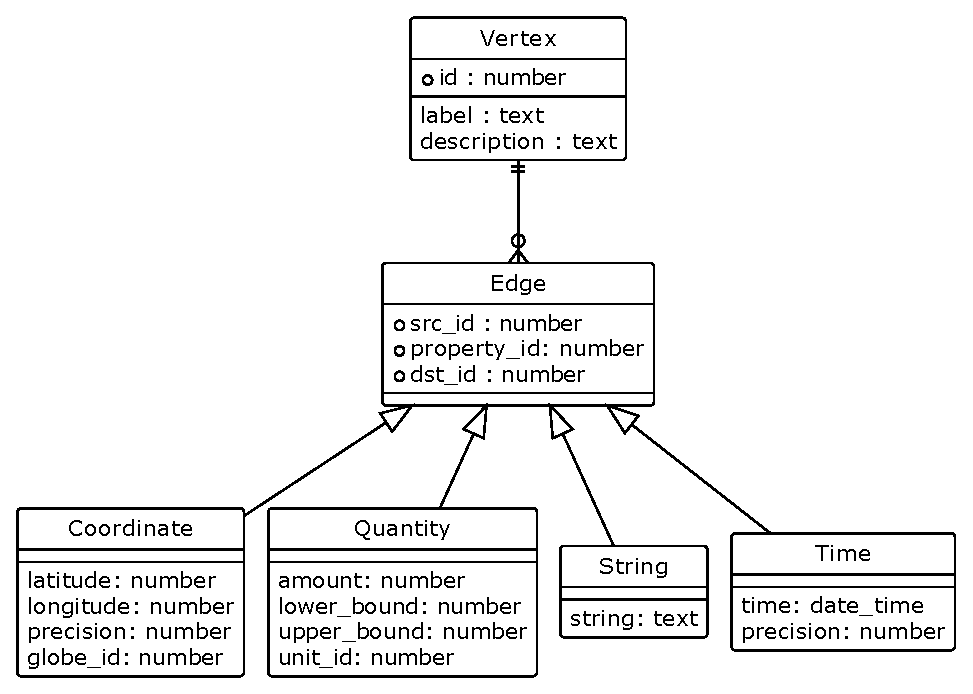
\includegraphics[width=.8\linewidth]{img/10-1_wd2duckdb.eps}
    \caption{Entity-relationship diagram of \texttt{wd2duckdb}'s resulting Database}
\end{figure}%

\chapter{A tool for validating Knowledge Graphs}
\label{chapter:pschema}
\epigraph{\textit{Logic is the foundation of the certainty of all the Knowledge we acquire.}}{-- \textup{Leonhard Euler}}

\section{Pregel-rs}

\section{PSchema-rs}

\part{Project Synthesis}

\chapter{Experimental Procedure}
\label{chapter:experiment}
\epigraph{\textit{No amount of experimentation can ever prove me right; a single experiment can prove me wrong.}}{-- \textup{Albert Einstein}}

\section{Methodology}

For us to evaluate the performance of our proposed method, we need to compare it with the state-of-the-art tools we showed in Chapter \ref{chapter:related}. For us to do so, we need to have a set of experiments that we can run on the same software environment. We also need to have a bunch of datasets that we can use to run the experiments. In this chapter, we will describe the methodology we used to conduct the experiments and the datasets we used to run them. For us to achieve this, we will answer the questions posed in Chapter \ref{chapter:intro}, namely, the project goals (see section \ref{section:objectives}).

\begin{enumerate}
    \itemsep0.5em
    \item To evaluate how the \textit{subsetting} tool has been improved, we need to run the \textit{subsetting} tool on the same software environment as the one used in the original paper. We will use the \textit{ETL} tool to compress the Wikidata JSON dump to a size that is manageable for the \textit{Pregel} algorithm. This is, we will try to tell if the tool has been improved in terms of the hardware needed to run it. Recall that for Labra's \cite{https://doi.org/10.48550/arxiv.2110.11709} solution to work, a costly machine with 4TB of RAM is required. We will verify if our solution can run on commodity hardware.
    \item To evaluate how the \textit{subsetting} tool has been improved, we need to measure the time it takes to subset the Wikidata JSON dump. We will compare the time it takes to subset the Wikidata JSON dump with the time it takes to subset the Wikidata JSON dump using the original tool.
    \item To evaluate how the \textit{subsetting} tool has been improved, we will try to subset other RDF datasets, apart from the Wikidata JSON dump. This is, we will try to tell if the tool is generic enough to subset other RDF Knowledge graphs.
\end{enumerate}

\section{Hardware}

For us to run the experiments, we need to have a machine with enough resources to run them. Hence, we will use a machine proprietary of the \textit{Web Semantic Research Group} (WESO) of the \textit{University of Oviedo}. The machine has the following specifications:

\begin{itemize}
    \itemsep0.5em
    \item \textbf{CPU}: Intel(R) Xeon(R) Silver 4214 CPU @ 2.20GHz (12 cores and 24 threads)
    \item \textbf{RAM}: 40GB
    \item \textbf{OS}: Ubuntu 20.04.3 LTS
\end{itemize}

\section{Datasets}

To test the above questions, we will use two types of datasets, namely, Wikidata JSON dumps and RDF datasets. We will use the Wikidata JSON dumps from 2017-08-21 to test the \textit{ETL} tool, and we will use both for the \textit{subsetting} tool. For us to compare our solution with the original one, we will use the same Wikidata JSON dump used in the original paper.

\chapter{Results and Analysis}
\label{chapter:results}
\epigraph{\textit{80\% of a piece of software can be written in 20\% of the total allocated time. Conversely, the hardest 20\% of the code takes 80\% of the time.}}{-- \textup{Roger S. Pressman}}

\section{\texttt{wd2duckdb}}

As we have seen in the previous chapter, the \texttt{wd2duckdb} tool is analyzed thoroughly for us to understand how it performs and what can be done to improve it. In this section, we will present the execution times of the tool provided several configurations. What we want to see is how the tool performs with different optimizations enabled and how it compares to the original version of the tool. As such, we will prove that the optimizations we have implemented are indeed useful and that they improve the performance of the tool. Recall that the optimizations that we have implemented were described in section \ref{section:optimizations}.

As can be seen in Figure \ref{fig:wd2duckdb}, the optimizations that we have implemented improve the performance of the tool. This is something that was expected before running the tests; however, the results obtained prove to be a worthy improvement. Note that for us to test the performance of the tool, we have used the same Wikidata dump for all the tests. The idea is to create 8 different databases each three times larger than the previous one. This, we have increased the number of Wikidata entities by a factor of 3 each time, starting from 10 thousand items to 21.87 million elements. This is, values in the abscissa axis
can be obtained through the following representation: $10,000 \cdot 3^n, n \in [0, 7]$. For us to fit such a big range of values in a single graph, we have used a logarithmic scale for the x-axis. This way, we can see the results of the tests in a single graph. Note that for the y-axis, we have used a linear scale, as the values are not that big, ranging from $0$ to $4,000$ and $40,000$ seconds, respectively, modeling the time it took to generate the database. This is said to be a \textit{semi-logarithmic} plot. To put it all together, we have used this type of representation to manage to test the tool with a wide range of values, and still, be able to see the results in a single graph.

For us to understand the values better, let me show them in a table, and then, we will comment on them in detail. Table \ref{table:wd2duckdb} shows the time it took to create the database with the different optimizations enabled and disabled.

\begin{figure}[p]
    \begin{subfigure}{0.49\textwidth}
        \centering
        \includestandalone[width=\textwidth,height=8cm]{diagrams/13-1_wd2duckdbOPT}
        \caption{Having all the optimizations enabled}
    \end{subfigure}%
    \hfill
    \begin{subfigure}{0.49\textwidth}
        \centering
        \includestandalone[width=\textwidth,height=8cm]{diagrams/13-2_wd2duckdbDEV}
        \caption{Having no optimization enabled}
    \end{subfigure}%
    \vspace*{1em}
    \begin{subfigure}{\textwidth}
        \centering
        \includestandalone[width=\textwidth]{diagrams/13-3_wd2duckdbBAR}
        \caption{Comparison between the two options: with and without optimizations}
    \end{subfigure}
    \caption{Time to create the database with \texttt{wd2duckdb}}
    \label{fig:wd2duckdb}
\end{figure}

\begin{table}[ht]
    \centering
    \begin{tabular}{|c|c|c|c|c|c|c|c|c|}
        \hline
        \rowcolor[HTML]{EFEFEF}
        \cellcolor[HTML]{C0C0C0}\textbf{N}               & \textit{0} & \textit{1} & \textit{2} & \textit{3} & \textit{4} & \textit{5} & \textit{6} & \textit{7} \\ \hline
        \cellcolor[HTML]{C0C0C0}\textbf{Optimizations}   & 4.56       & 11.05      & 26.36      & 54.87      & 112.30     & 250.86     & 1,349.10   & 3,730.33   \\ \hline
        \cellcolor[HTML]{C0C0C0}\textbf{No Optimization} & 40.18      & 99.52      & 243.64     & 514.68     & 1,081.64   & 2,566.25   & 13,157.18  & 37,340.60  \\ \hline
    \end{tabular}
    \caption{Time to create the database with \texttt{wd2duckdb}}
    \label{table:wd2duckdb}
\end{table}

As can be seen, the time it takes \texttt{wd2duckdb} to process the dumps grows at a linear rate. What's more, we can see that the speedup in the execution time is almost 10. Let me first calculate this value, and then, we will comment on the results. Having ${Time_{DEV}}_i$ the $i^{th}$ execution time of the tool in developer mode, that is, with no optimization enabled, and ${Time_{OPT}}_j$ the $j^{th}$ execution time of the tool in release mode, that is, with all the optimizations enabled. The speedup is calculated as follows:

\begin{equation}
    \text{Speedup} = \frac{\overline{Time_{DEV}}}{\overline{Time_{OPT}}} = \frac{\sum_{i=0}^{7}t_i}{\sum_{j=0}^{7}t_j} = \frac{40.18 + \cdots + 37,340.60}{4.56 + \cdots + 3,730.33} = \frac{55,043.70}{5,539.43} = 9.94
\end{equation}

Regarding the size of the database resulting from the execution of the algorithm, it is worth noting that it is hard to compare it to the size of the original dump, as not only the compression rate has an impact on the size of the database, but also the number of columns that we have decided to store, as well as the language chosen for the labels and descriptions. However, we can see that the size of the database is around 10 times smaller than the original dump. To put it into perspective, the size of the original dump is  224.24 GB uncompressed, and 16.94 GB compressed. While the size of the database is 9.38 GB. This means that the database is 23.9 times smaller than the original dump and 1.6 times smaller than the compressed dump. Even though we cannot state that there's a fixed compression rate, we can say that the resulting database is smaller than the original dump. Hence, we can say that the algorithm is efficient in terms of space.

Regarding the complexity of the algorithm, we can say that it is linear. This is because the algorithm iterates over the whole dump, and for each line, it performs a constant number of operations, mainly parsing and inserting a certain Wikidata entity. Hence, the complexity of the algorithm is $O(n)$, where $n$ is the number of lines in the dump. This is also the reason why the time it takes to create the database grows linearly with the size of the dump. This has been proved empirically in the experiment conducted. Refer to Figure \ref{fig:wd2duckdb} for more information.

\section{\texttt{pschema-rs}}

In this section, we will analyze the results obtained from the execution of \texttt{pschema-rs}. Recall that the experiment conducted will be focused on three aspects: the time it takes to create the subsets of Wikidata, the resources used during the execution of the algorithm, and the possibility of creating subsets from other RDF datasets.

The first thing we will analyze is the time it takes to create the subsets of Wikidata. For us to do so, we will execute the algorithm three times, each of them with the same configuration and the same subset of Wikidata, the one of the $21^{st}$ August 2017. Then, we will calculate the average time it takes to create the subsets. Apart from that, we will also track the memory used during the execution of the algorithm. Hence, we will see if it is feasible to create subsets of Wikidata in a machine with acceptable resources. What I mean by this is that we will see if it is possible to create subsets of Wikidata in a machine that, even if it has some resources, is not a supercomputer. Finally, we will compare the results obtained with the ones obtained by \texttt{wdsub}, the tool that we have used as a baseline and that we have described in Section \ref{section:wd2sub}. It is worth noting that this tool is the recommendation of the Wikidata community to create subsets of Wikidata. Hence, we will see if the tool that we have developed is faster than the one recommended by the community.

\begin{table}[ht]
    \centering
    \begin{tabular}{|
            >{\columncolor[HTML]{C0C0C0}}c|c|c|c|c|}
        \hline
        \textbf{N}          & \cellcolor[HTML]{EFEFEF}\textit{0} & \cellcolor[HTML]{EFEFEF}\textit{1} & \cellcolor[HTML]{EFEFEF}\textit{2} & \cellcolor[HTML]{EFEFEF}\textbf{Memory (GB)} \\ \hline
        \textbf{pschema-rs} & 5,014.34                           & 4,995.30                           & 4,996.04                           & 20.3                                         \\ \hline
        \textbf{wdsub}      & 5,090.01                           & 5,064.14                           & 5,071.09                           & -                                            \\ \hline
    \end{tabular}
    \caption{Time to create the \textit{subsets} of Wikidata with \texttt{pschema-rs} and \texttt{wdsub}}
    \label{table:pschema-rs}
\end{table}

As can be seen in table \ref{table:pschema-rs}, both solutions take a similar time to create the subsets of Wikidata. However, we can see that \texttt{pschema-rs} is slightly faster than \texttt{wdsub}. Let me first calculate the speedup, and then, we will comment on the results.

\begin{equation}
    \text{Speedup} = \frac{\overline{Time_{wdsub}}}{\overline{Time_{pschema-rs}}} = \frac{\sum_{i=0}^{2}t_i}{\sum_{j=0}^{2}t_j} = \frac{5,090.01 + \cdots + 5,071.09}{5,014.34 + \cdots + 4,996.04} = \frac{15,225.28}{15,005.69} = 1.01
\end{equation}

As can be seen, the speedup is slightly higher than 1. This means that \texttt{pschema-rs} is slightly faster than \texttt{wdsub}. However, we can see that the difference is not significant. However, far from letting us down, this result is encouraging. Recall that \texttt{wdsub} is a mature tool, while we are still in the early stages of development. Hence, we can say that the results obtained are promising. Moreover, we can see that the memory used by \texttt{pschema-rs} is around 20 GB. This means that it is possible to create subsets of Wikidata in a machine with acceptable resources. Hence, we can say that the algorithm is efficient in terms of time and memory. Having said that, we will now analyze the results obtained from the execution of the algorithm with other RDF datasets.

Before getting into more details, let me define what I mean by \texttt{DEV} and \texttt{OPT}. Recall that in section \ref{section:pschema-rs:optimizations} we showed two main optimizations that we would take advantage from.

\begin{table}[ht]
    \centering
    \begin{tabular}{c|
            >{\columncolor[HTML]{EFEFEF}}c |c|c|c|c|}
        \cline{2-6}
                                                                                     & \cellcolor[HTML]{C0C0C0}\textbf{Shape Expression} & \cellcolor[HTML]{C0C0C0}\textbf{Initial triples} & \cellcolor[HTML]{C0C0C0}\textbf{Resulting triples} & \cellcolor[HTML]{C0C0C0}\textbf{Time (s)} & \cellcolor[HTML]{C0C0C0}\textbf{Memory (GB)} \\ \hline
        \multicolumn{1}{|c|}{\cellcolor[HTML]{C0C0C0}}                               & \texttt{protein}                                  & 7,346,129                                        & 226,241                                            & 23.35                                     & 6.74                                         \\ \cline{2-6}
        \multicolumn{1}{|c|}{\multirow{-2}{*}{\cellcolor[HTML]{C0C0C0}\textbf{DEV}}} & \texttt{subcellular\_location}                    & 7,346,129                                        & 1,084,151                                          & 57.56                                     & 6.04                                         \\ \hline
        \multicolumn{1}{|c|}{\cellcolor[HTML]{C0C0C0}}                               & \texttt{protein}                                  & 7,346,129                                        & 226,241                                            & 14.58                                     & 3.87                                         \\ \cline{2-6}
        \multicolumn{1}{|c|}{\multirow{-2}{*}{\cellcolor[HTML]{C0C0C0}\textbf{OPT}}} & \texttt{subcellular\_location}                    & 7,346,129                                        & 1,084,151                                          & 37.76                                     & 3.75                                         \\ \hline
    \end{tabular}
    \caption{Time and memory consumption to create the \textit{subsets} of \texttt{Uniprot} with \texttt{pschema-rs}}
    \label{tab:my-table}
\end{table}

\begin{figure}[p]
    \begin{subfigure}{\textwidth}
        \centering
        \includestandalone[width=\textwidth,height=6cm]{diagrams/13-4_pschemaN}
        \caption{Modifying the number of Wikidata Entities}
    \end{subfigure}%
    \vspace*{1em}
    \begin{subfigure}{\textwidth}
        \centering
        \includestandalone[width=\textwidth,height=6cm]{diagrams/13-5_pschemaDEPTH}
        \caption{Modifying the depth of the \texttt{ShEx} tree}
    \end{subfigure}%
    \vspace*{1em}
    \begin{subfigure}{\textwidth}
        \centering
        \includestandalone[width=\textwidth,height=6cm]{diagrams/13-6_pschemaBREADTH}
        \caption{Modifying the breadth of the \texttt{ShEx} tree}
    \end{subfigure}
    \caption{Time to create the \textit{subsets} of Wikidata with \texttt{pschema-rs}}
\end{figure}

\chapter{Planning and Budget}
\label{chapter:planning}
\epigraph{\textit{Give me six hours to chop down a tree and I will spend the first four sharpening the axe.}}{-- \textup{Abraham Lincoln}}

\section{Planning}

This project's planning was divided into four main phases: the first one was the \textbf{research phase}, where the state of the art was studied and the main concepts were understood; the second one was the \textbf{development phase}, where the main focus was to develop the project's solution; to continue, the \textbf{writing phase} was the period at which the thesis was written. Lastly, the last part of this project is the \textbf{defense of the work phase}, where the thesis is presented and defended. Thus, we can see the project's timeline in \ref{fig:summary_timeline}, for a more detailed description, see Figure \ref{fig:timeline} and Table \ref{tab:timeline}.

\begin{figure}[ht]
    \centering
    \includestandalone[width=1\textwidth]{diagrams/14-2_summary}
    \caption{Project timeline highlighting the most important reached milestones}
    \label{fig:summary_timeline}
\end{figure}

\subsection{Research phase}

The research phase was divided into two main parts: the first one was the \textbf{research of the state of the art}, where the main concepts were studied and understood; the second one was the \textbf{research of the technologies}, where the technologies that were going to be used in the project were analyzed. To be fair, part of this phase was done during the development phase, as we changed the technologies that were going to be used in the project. However, the main concepts were already understood, so the research on the technologies was not that hard. Hence, we can say that the research phase ended when the development phase started. Following the naming convention used, this phase includes the \textit{Literature review} and the \textit{Learning new technologies} stages.

\subsection{Development phase}

The development phase was divided into three main parts: the first one was the \textbf{development of DataFrame-based solution}, where we tried to develop a solution based on DataFrames. As have already discussed, the outcome of this part was not as expected, so we had to change the approach; the second one was the \textbf{development of the ETL pipeline}, where we developed the \texttt{wd2duckdb} tool; the third one was the \textbf{development of the Pregel algorithm}, where we developed the \texttt{pschema-rs} tool. Following the naming convention used, this phase includes the \textit{Proposed Solution Development} stage.

\subsection{Writing phase}

The writing phase was divided into two main parts: the first one was the \textbf{literature review}, where the state of the art was studied and written; the second one was the \textbf{thesis}, where the thesis was written. The first part was done during the research phase; for the sake of simplicity, we will consider that the \textit{literature review} stage is part of the \textit{research phase}. Hence, the writing phase is only composed of the \textit{thesis} stage, where I wrote the part of the thesis that is created entirely by me. Following the naming convention used, this phase includes the \textit{Dissertation Document} stage.

\subsection{Defense of the work phase}

The defense of the work phase was divided into two main parts: the first one was the \textbf{presentation of the thesis}, where the slides and the presentation were created; the second one was the \textbf{defense of the thesis}, where the thesis is going to be presented and defended. This part has not been done yet; however, it is already planned. Following the naming convention used, this phase includes the \textit{Defense of the project} stage.

\subsection{Other phase}

We have also included another phase, namely, the \textbf{meetings phase}, where the meetings with the tutor were held. Following the naming convention used, this phase includes the \textit{Meetings} stage.

The time spent in each phase is shown in Figure \ref{fig:pie}. The project's timeline is shown in Figure \ref{fig:timeline} and Table \ref{tab:timeline}. Note that the project's timeline is not a Gantt chart, as it does not show the dependencies between the tasks. However, it is a good way to show the project's timeline. The project's budget is shown in Table \ref{table:costs}.

\begin{figure}[ht]
    \centering
    \begin{adjustbox}{max width=0.66\textwidth}
        \begin{tikzpicture}
            \pie[hide number]{
                1.41/Meetings (1.41\%),
                7.93/Literature Review (7.93\%),
                41.56/Dissertation Document (41.56\%),
                37.78/Proposed Solution Development (37.78\%),
                7.55/Learning new technologies (7.55\%),
                3.77/Defense of the project (3.77\%)
            }
        \end{tikzpicture}
    \end{adjustbox}
    \caption{Part of the project's budget spent in each phase}
    \label{fig:pie}
\end{figure}

\begin{figure}[p]
    \centering
    \includestandalone[width=1\textwidth]{diagrams/14-1_timeline}
    \caption{Project timeline highlighting all the reached milestones}
    \label{fig:timeline}
\end{figure}

\begin{table}[p]
    \centering
    \documentclass{standalone}
\usepackage[table,xcdraw]{xcolor}
\usepackage{varioref,multicol}
\usepackage{hyperref}  
\begin{document}
\begin{tabular}{|r|llll|}
    \hline
    \rowcolor[HTML]{C0C0C0}
    \multicolumn{1}{|c|}{\cellcolor[HTML]{C0C0C0}\textbf{ID}}     & \multicolumn{1}{c|}{\cellcolor[HTML]{C0C0C0}\textbf{Task name}} & \multicolumn{1}{c|}{\cellcolor[HTML]{C0C0C0}\textbf{Duration}} & \multicolumn{1}{c|}{\cellcolor[HTML]{C0C0C0}\textbf{Start}} & \multicolumn{1}{c|}{\cellcolor[HTML]{C0C0C0}\textbf{Finish}} \\ \hline
    \textbf{1}                                                    & \multicolumn{4}{c|}{\textit{Meetings}}                                                                                                                                                                                                                        \\ \hline
    1.1                                                           & \multicolumn{1}{l|}{Project's first meeting}                    & \multicolumn{1}{l|}{1 hour}                                    & \multicolumn{1}{l|}{Fri 16 September, 2022}                 & Fri 16 September, 2022                                       \\ \hline
    1.2                                                           & \multicolumn{1}{l|}{Project's second meeting}                   & \multicolumn{1}{l|}{2.5 hours}                                 & \multicolumn{1}{l|}{Thu 29 September, 2022}                 & Thu 29 September, 2022                                       \\ \hline
    1.3                                                           & \multicolumn{1}{l|}{Project's third meeting}                    & \multicolumn{1}{l|}{2 hours}                                   & \multicolumn{1}{l|}{Mon 20 February, 2023}                  & Mon 20 February, 2023                                        \\ \hline
    \textbf{2}                                                    & \multicolumn{4}{c|}{\textit{Literature Review}}                                                                                                                                                                                                               \\ \hline
    2.1                                                           & \multicolumn{1}{l|}{Knowledge graphs}                           & \multicolumn{1}{l|}{5 hours}                                   & \multicolumn{1}{l|}{Thu 29 September, 2022}                 & Fri 30 September, 2022                                       \\ \hline
    2.2                                                           & \multicolumn{1}{l|}{Wikibase graphs}                            & \multicolumn{1}{l|}{10 hours}                                  & \multicolumn{1}{l|}{Fri 30 September, 2022}                 & Sat 15 October, 2022                                         \\ \hline
    2.3                                                           & \multicolumn{1}{l|}{Knowledge Graph validation}                 & \multicolumn{1}{l|}{7 hours}                                   & \multicolumn{1}{l|}{Sat 29 October, 2022}                   & Sat 5 November, 2022                                         \\ \hline
    2.4                                                           & \multicolumn{1}{l|}{Knowledge Graph Subsetting}                 & \multicolumn{1}{l|}{0.5 hours}                                 & \multicolumn{1}{l|}{Mon 7 November, 2022}                   & Mon 7 November, 2022                                         \\ \hline
    2.5                                                           & \multicolumn{1}{l|}{MapReduce}                                  & \multicolumn{1}{l|}{3 hours}                                   & \multicolumn{1}{l|}{Tue 4 October, 2022}                    & Tue 4 October, 2022                                          \\ \hline
    2.6                                                           & \multicolumn{1}{l|}{Pregel system}                              & \multicolumn{1}{l|}{6 hours}                                   & \multicolumn{1}{l|}{Tue 4 October, 2022}                    & Thu 6 October, 2022                                          \\ \hline
    \textbf{3}                                                    & \multicolumn{4}{c|}{\textit{Dissertation Document}}                                                                                                                                                                                                           \\ \hline
    3.1                                                           & \multicolumn{1}{l|}{Introduction}                               & \multicolumn{1}{l|}{5 hours}                                   & \multicolumn{1}{l|}{Wed 9 November, 2022}                   &                                                              \\ \hline
    3.2                                                           & \multicolumn{1}{l|}{Related Work}                               & \multicolumn{1}{l|}{3 hours}                                   & \multicolumn{1}{l|}{Fri 11 November, 2022}                  &                                                              \\ \hline
    3.3                                                           & \multicolumn{1}{l|}{Theoretical Background}                     & \multicolumn{1}{l|}{45 hours}                                  & \multicolumn{1}{l|}{Thu 29 September, 2022}                 &                                                              \\ \hline
    3.4                                                           & \multicolumn{1}{l|}{Analysis of the Initial solution}           & \multicolumn{1}{l|}{10 hours}                                  & \multicolumn{1}{l|}{Fri 11 November, 2022}                  &                                                              \\ \hline
    3.5                                                           & \multicolumn{1}{l|}{The DataFrame-based solution}               & \multicolumn{1}{l|}{10 hours}                                  & \multicolumn{1}{l|}{Fri 11 November, 2022}                  &                                                              \\ \hline
    3.6                                                           & \multicolumn{1}{l|}{Analysis of the Rust solution}              & \multicolumn{1}{l|}{10 hours}                                  & \multicolumn{1}{l|}{Fri 11 November, 2022}                  &                                                              \\ \hline
    3.7                                                           & \multicolumn{1}{l|}{The ETL pipeline}                           & \multicolumn{1}{l|}{10 hours}                                  & \multicolumn{1}{l|}{Fri 11 November, 2022}                  &                                                              \\ \hline
    3.8                                                           & \multicolumn{1}{l|}{The subsetting tool}                        & \multicolumn{1}{l|}{10 hours}                                  & \multicolumn{1}{l|}{Fri 11 November, 2022}                  &                                                              \\ \hline
    3.9                                                           & \multicolumn{1}{l|}{Experimental Procedure}                     & \multicolumn{1}{l|}{}                                          & \multicolumn{1}{l|}{}                                       &                                                              \\ \hline
    3.10                                                          & \multicolumn{1}{l|}{Results and Analysis}                       & \multicolumn{1}{l|}{}                                          & \multicolumn{1}{l|}{}                                       &                                                              \\ \hline
    3.11                                                          & \multicolumn{1}{l|}{Planning and Budget}                        & \multicolumn{1}{l|}{}                                          & \multicolumn{1}{l|}{Thu 20 October, 2022}                   &                                                              \\ \hline
    3.12                                                          & \multicolumn{1}{l|}{Conclusions}                                & \multicolumn{1}{l|}{}                                          & \multicolumn{1}{l|}{}                                       &                                                              \\ \hline
    \textbf{4}                                                    & \multicolumn{4}{c|}{\textit{Proposed Solution Development}}                                                                                                                                                                                                   \\ \hline
    4.1                                                           & \multicolumn{1}{l|}{The DataFrame-based solution}               & \multicolumn{1}{l|}{30 hours}                                  & \multicolumn{1}{l|}{Sun 29 January, 2023}                   & Mon 20 February, 2023                                        \\ \hline
    4.2                                                           & \multicolumn{1}{l|}{\texttt{wd2duckdb}}                         & \multicolumn{1}{l|}{}                                          & \multicolumn{1}{l|}{Tue 21 February, 2023}                  &                                                              \\ \hline
    4.3                                                           & \multicolumn{1}{l|}{\texttt{pregel-rs}}                         & \multicolumn{1}{l|}{}                                          & \multicolumn{1}{l|}{Tue 21 February, 2023}                  &                                                              \\ \hline
    4.4                                                           & \multicolumn{1}{l|}{\texttt{pschema-rs}}                        & \multicolumn{1}{l|}{}                                          & \multicolumn{1}{l|}{Tue 21 February, 2023}                  &                                                              \\ \hline
    \textbf{5}                                                    & \multicolumn{4}{c|}{\textit{Learning new technologies}}                                                                                                                                                                                                       \\ \hline
    5.1                                                           & \multicolumn{1}{l|}{Scala}                                      & \multicolumn{1}{l|}{10 hours}                                  & \multicolumn{1}{l|}{Tue 6 December, 2022}                   & Tue 27 December, 2022                                        \\ \hline
    5.2                                                           & \multicolumn{1}{l|}{Apache Spark}                               & \multicolumn{1}{l|}{5 hours}                                   & \multicolumn{1}{l|}{Thu 29 December, 2022}                  & Sat 7 January, 2023                                          \\ \hline
    5.3                                                           & \multicolumn{1}{l|}{Rust}                                       & \multicolumn{1}{l|}{5 hours}                                   & \multicolumn{1}{l|}{Tue 21 February, 2023}                  &                                                              \\ \hline
    5.4                                                           & \multicolumn{1}{l|}{DuckDB}                                     & \multicolumn{1}{l|}{5 hours}                                   & \multicolumn{1}{l|}{Tue 21 February, 2023}                  &                                                              \\ \hline
    5.5                                                           & \multicolumn{1}{l|}{Pola-rs}                                    & \multicolumn{1}{l|}{5 hours}                                   & \multicolumn{1}{l|}{Tue 21 February, 2023}                  &                                                              \\ \hline
    \textbf{6}                                                    & \multicolumn{4}{c|}{\textit{Defense of the project}}                                                                                                                                                                                                          \\ \hline
    6.1                                                           & \multicolumn{1}{l|}{Keynote document}                           & \multicolumn{1}{l|}{10 hours}                                  & \multicolumn{1}{l|}{Tue 6 December, 2022}                   & Tue 27 December, 2022                                        \\ \hline
    6.2                                                           & \multicolumn{1}{l|}{Preparation of the speech}                  & \multicolumn{1}{l|}{5 hours}                                   & \multicolumn{1}{l|}{Thu 29 December, 2022}                  & Sat 7 January, 2023                                          \\ \hline
    \multicolumn{2}{|r|}{\cellcolor[HTML]{C0C0C0}\textbf{Total:}} & \multicolumn{1}{l|}{159 hours}                                                                                                                                                                                                                                \\ \cline{1-3}
\end{tabular}
\end{document}
    \caption{Tasks planning of the project}
    \label{tab:timeline}
\end{table}

\section{Budget}

Note that part of this project was done during an internship at \textit{WESO}. Hence, the budget for this project is going to be calculated based on the rate that the \textit{University of Oviedo} pays to its interns\footnote{\url{https://www.funiovi.org/estudiantes/practicas}}. Provided a 20 hours per week internship, the maximum wage is 400€ per month. Hence, given that a work month has 4.33 weeks, the hourly rate is 4.61€. This rate is going to be used to calculate the budget of this project.

For us to calculate the budget, we need to know two main aspects. First, we need to know the sum of the \textit{Indirect costs}, which are the costs that even though they are not directly related to the project, are necessary for the project to be done. Second, we need to know the sum of the \textit{Direct costs}, which are the costs that are directly related to the project. This is the sum of the costs of each of the phases of the project. Let me start by explaining the \textit{Indirect costs}.

\subsection{Indirect costs}

The \textit{Indirect costs} of this project is divided into two main parts: the \textbf{costs of the means of production} and the \textbf{rest of Indirect costs}. The first one is the cost associated with the means of production, such as the computer, the software, the licenses, etc. The second one is the cost associated with the rest of the \textit{Indirect costs}, such as electricity, Internet, etc. The \textit{Indirect costs} are shown in Table \ref{table:indirect-costs}. It is worth noting that the \textit{Indirect costs} are calculated based on some general approximations. For example, the cost of the computer is calculated based on the average price of a computer with similar characteristics. The cost of the \textit{rest of Indirect cost} is rounded as it is not possible to know the exact cost of each of the items. Recall, this project was performed at my home, so the \textit{rest of Indirect cost} is calculated based on the cost of the electricity and the Internet at my home, and the impact of the project on the electricity and the Internet bill.

\begin{figure}[ht]
    \begin{subfigure}{\textwidth}
        \centering
        \begin{tabular}{|cccccc|}
            \hline
            \rowcolor[HTML]{C0C0C0}
            \multicolumn{6}{|c|}{\cellcolor[HTML]{C0C0C0}\textbf{Costs of the means of production}}                                                                                                                                                                                                                                                                 \\ \hline
            \rowcolor[HTML]{EFEFEF}
            \multicolumn{1}{|c|}{\cellcolor[HTML]{EFEFEF}\textit{Component / License}} & \multicolumn{1}{c|}{\cellcolor[HTML]{EFEFEF}\textit{Units}} & \multicolumn{1}{c|}{\cellcolor[HTML]{EFEFEF}\textit{Cost}} & \multicolumn{1}{c|}{\cellcolor[HTML]{EFEFEF}\textit{Total Costs}} & \multicolumn{1}{c|}{\cellcolor[HTML]{EFEFEF}\textit{Type}} & \textit{Terms} \\ \hline
            \multicolumn{1}{|c|}{Development Systems}                                  & \multicolumn{1}{c|}{1}                                      & \multicolumn{1}{c|}{1,500.00 €}                            & \multicolumn{1}{c|}{1,500.00 €}                                   & \multicolumn{1}{c|}{Amortization}                          & 1              \\ \hline
            \multicolumn{1}{|c|}{Server\footnotemark}                                  & \multicolumn{1}{c|}{1}                                      & \multicolumn{1}{c|}{3,565.79 €}                            & \multicolumn{1}{c|}{3,565.79 €}                                   & \multicolumn{1}{c|}{Amortization}                          & 1              \\ \hline
            \multicolumn{3}{|c|}{\cellcolor[HTML]{C0C0C0}\textbf{Total}}               & \multicolumn{3}{c|}{5,065.79 €}                                                                                                                                                                                                                                            \\ \hline
        \end{tabular}
        \caption{Costs of the means of production}
    \end{subfigure}%
    \vspace*{1em}
    \begin{subfigure}{\textwidth}
        \centering
        \begin{tabular}{|ccc|}
            \hline
            \rowcolor[HTML]{C0C0C0}
            \multicolumn{3}{|c|}{\cellcolor[HTML]{C0C0C0}\textbf{Indirect costs}}                                                                                      \\ \hline
            \rowcolor[HTML]{EFEFEF}
            \multicolumn{1}{|c|}{\cellcolor[HTML]{EFEFEF}\textit{Service}} & \multicolumn{1}{c|}{\cellcolor[HTML]{EFEFEF}\textit{Monthly Cost}} & \textit{Annual Cost} \\ \hline
            \multicolumn{1}{|c|}{Natural Gaz}                              & \multicolumn{1}{c|}{10.00 €}                                       & 110.00 €             \\ \hline
            \multicolumn{1}{|c|}{Electricity}                              & \multicolumn{1}{c|}{20.00 €}                                       & 220.00 €             \\ \hline
            \multicolumn{1}{|c|}{Water}                                    & \multicolumn{1}{c|}{5.00 €}                                        & 55.00 €              \\ \hline
            \multicolumn{1}{|c|}{Telecommunications}                       & \multicolumn{1}{c|}{30.00 €}                                       & 330.00 €             \\ \hline
            \multicolumn{1}{|c|}{\cellcolor[HTML]{C0C0C0}\textbf{Total}}   & \multicolumn{2}{c|}{715.00 €}                                                             \\ \hline
        \end{tabular}
        \caption{Costs that are not direct to the project, but are required for us to work}
    \end{subfigure}%
    \caption{Indirect costs}
    \label{table:indirect-costs}
\end{figure}
\footnotetext{\url{https://www.pccomponentes.com/hpe-proliant-ml350-gen10-intel-xeon-silver-4214r-32gb}}

\subsection{Final Budget}

The final budget of the project is the sum of the direct costs, calculated as the time it takes to complete every phase, as seen in the previous section, times the hourly rate, the indirect costs and the costs of the means of production. We have also considered a 21\% VAT on the total amount of the project. Note that as this is a research project, the profit margin is 0\%, as the project is not intended to be sold, and the benefit we take from it is the knowledge acquired and the resulting code and documentation.

\begin{table}[p]
    \renewcommand{\arraystretch}{1.5}
    \setlength{\tabcolsep}{.25cm}
    \centering
    \begin{tabular}{|clcc|}
        \hline
        \rowcolor[HTML]{C0C0C0}
        \multicolumn{2}{|c|}{\cellcolor[HTML]{C0C0C0}\textbf{Phase}}               & \multicolumn{1}{c|}{\cellcolor[HTML]{C0C0C0}\textbf{Hours}} & \textbf{Total cost} \\ \hline
        \multicolumn{2}{|c|}{Research}                                             & \multicolumn{1}{c|}{61.5}                                   & 283.52 €            \\ \hline
        \multicolumn{2}{|c|}{Development}                                          & \multicolumn{1}{c|}{150}                                    & 691.50 €            \\ \hline
        \multicolumn{2}{|c|}{Writing}                                              & \multicolumn{1}{c|}{165}                                    & 760.65 €            \\ \hline
        \multicolumn{2}{|c|}{Defense of the Work}                                  & \multicolumn{1}{c|}{15}                                     & 69.15 €             \\ \hline
        \multicolumn{2}{|c|}{Other}                                                & \multicolumn{1}{c|}{5.5}                                    & 25.36 €             \\ \hline
        \rowcolor[HTML]{EFEFEF}
        \multicolumn{4}{|l|}{\cellcolor[HTML]{EFEFEF}}                                                                                                                 \\ \hline
        \multicolumn{3}{|r|}{Project Costs}                                        & 1,830.18 €                                                                        \\ \hline
        \multicolumn{3}{|r|}{Total Indirect Costs}                                 & 5,780.79 €                                                                        \\ \hline
        \multicolumn{2}{|r|}{Taxes}                                                & \multicolumn{1}{c|}{21\%}                                   & 405.34 €            \\ \hline
        \rowcolor[HTML]{EFEFEF}
        \multicolumn{4}{|l|}{\cellcolor[HTML]{EFEFEF}}                                                                                                                 \\ \hline
        \multicolumn{3}{|r|}{\cellcolor[HTML]{C0C0C0}\textbf{Project Total Costs}} & 8,016.31 €                                                                        \\ \hline
    \end{tabular}
    \caption{Aggregated costs of the whole project}
    \label{table:costs}
\end{table}


\chapter{Conclusions}
\label{chapter:conclusions}
\epigraph{\textit{The programmers of tomorrow are the wizards of the future. You're going to look like you have magic powers compared to everybody else.}}{-- \textup{Gabe Newell}}

\section{Achievements}

From June the $25^{th}$ to July the $1^{st}$, the \textit{DBCLS BioHackathon 2023} took place, this is an event focused on the standardization and interoperability of life sciences and biomedical databases, namely, Knowledge Graphs. Following this, during the event, the tool presented in this project was used to create some subsets of the \textit{Uniprot} database. Which was later published in the \textit{Zenodo} repository, and can be found in the following link: \url{https://zenodo.org/record/8086938}.

\section{Future work}

The tool presented in this project is still in its early stages, and many improvements can be made to it. Some of the most important ones are:

\begin{enumerate}
    \itemsep0.5em
    \item \textbf{Improve the performance of the tool}: The tool is still slow, and it can be improved by using a more efficient programming language, or by using a more efficient algorithm.
    \item \textbf{Add more features}: The tool can be improved by adding more features, such as the ability to create subsets of the database based on the taxonomy of the proteins.
\end{enumerate}

Apart from the improvements that I have just mentioned, several other use cases can be implemented using the tool presented in this project. Some of the most important ones are:

\section{Personal opinion}

\part{Annexes and References}

\appendix
\chapter{Execution of a \texttt{pregel-rs} algorithm}
\label{appendix:trace}
\input{thesis_appx01_trace}

\chapterimage{img/misc/heading_bib.jpg} % Chapter heading image
\chapter{References} % Chapter heading image
\printbibliography[heading=bibempty]

\end{document}